\documentclass[12pt, a4paper]{report}
% ── Packages ──────────────────────────────────────────────────────────────────
\usepackage[a4paper, top=3.1cm, bottom=2.5cm, left=3.0cm, right=1.0cm]{geometry}
\usepackage[T1]{fontenc}
\usepackage[utf8]{inputenc}
\usepackage{mathptmx}
\usepackage{setspace}
\usepackage{parskip}
\setlength{\parskip}{5pt}
\setlength{\parindent}{0pt}
\usepackage{titlesec}
\usepackage{booktabs}
\usepackage{array}
\usepackage{xcolor}
\usepackage{hyperref}
\usepackage{graphicx}
\usepackage{float}
\usepackage{caption}
\usepackage{enumitem}
\usepackage{fancyhdr}
\usepackage{amsmath}
\usepackage{amssymb}
\usepackage{microtype}
\usepackage{tocloft}
\usepackage{listings}
\usepackage{subcaption}
\usepackage{algorithm}
\usepackage{algpseudocode}
\usepackage{needspace}
\usepackage{tikz}
\usetikzlibrary{shapes.geometric, arrows.meta, positioning, fit, backgrounds}
\hypersetup{colorlinks=true,linkcolor=black,citecolor=black,urlcolor=black}
\setlength{\headheight}{14pt}
\titleformat{\chapter}[block]
  {\fontsize{24pt}{28pt}\selectfont\bfseries}{\thechapter.}{0.5em}{}
\titleformat{\section}
  {\fontsize{17pt}{21pt}\selectfont\bfseries}{\thesection}{0.5em}{}
\titleformat{\subsection}
  {\fontsize{14pt}{18pt}\selectfont\bfseries}{\thesubsection}{0.5em}{}
\titleformat{\subsubsection}
  {\fontsize{12pt}{16pt}\selectfont\bfseries}{\thesubsubsection}{0.5em}{}
\titlespacing{\chapter}{0pt}{0pt}{12pt}
\titlespacing{\section}{0pt}{16pt}{6pt}
\titlespacing{\subsection}{0pt}{12pt}{4pt}
\titlespacing{\subsubsection}{0pt}{10pt}{4pt}
\setstretch{1.15}
\pagestyle{fancy}
\fancyhf{}
\fancyhead[L]{\small Black-Box Membership Inference in Federated Learning}
\fancyhead[R]{}
\fancyfoot[C]{\small\thepage}
\renewcommand{\headrulewidth}{0.4pt}
\newcolumntype{L}[1]{>{\raggedright\arraybackslash}p{#1}}
\newcolumntype{C}[1]{>{\centering\arraybackslash}p{#1}}
\captionsetup{font=small, labelfont=bf, labelsep=period}
\renewcommand{\arraystretch}{1.15}
\setlength{\tabcolsep}{6pt}
\setlength{\textfloatsep}{14pt plus 2pt minus 2pt}
\setlength{\floatsep}{14pt plus 2pt minus 2pt}
\setlength{\intextsep}{14pt plus 2pt minus 2pt}
\lstset{
  basicstyle=\ttfamily\footnotesize,
  breaklines=true,
  frame=single,
  numbers=left,
  numberstyle=\tiny,
  xleftmargin=15pt,
}

% ── TikZ colour definitions ───────────────────────────────────────────────────
\definecolor{tealcolor}{RGB}{13,148,136}
\definecolor{navycolor}{RGB}{13,27,42}
\definecolor{bluecolor}{RGB}{55,138,221}
\definecolor{redcolor}{RGB}{239,68,68}
\definecolor{goldcolor}{RGB}{245,158,11}
\definecolor{lightgray}{RGB}{240,244,248}

% ══════════════════════════════════════════════════════════════════════════════
\begin{document}
% ── Title page ────────────────────────────────────────────────────────────────
\begin{titlepage}
  \centering
  \vspace*{1cm}
  {\large Eötvös Loránd University\par}
  \vspace{0.2cm}
  {\large Faculty of Informatics\par}
  \vspace{0.2cm}
  {\normalsize Department of Data Science and Engineering\par}
  \vspace{3.5cm}
  {\fontsize{22pt}{28pt}\selectfont\bfseries
    Evaluating Black-Box Membership\\[8pt]
    Inference Attacks in Federated\\[8pt]
    Learning Systems\par}
  \vspace{4cm}
  \begin{tabular}{p{6cm} p{6cm}}
    \textit{Supervisor:}  & \textit{Author:} \\[6pt]
    Kiss Péter            & Abdihakim Yussuf Abdi \\
                          & Data Science MSc \\
  \end{tabular}
  \vfill
  {\normalsize Budapest, 2026\par}
\end{titlepage}

% ── Abstract ──────────────────────────────────────────────────────────────────
\chapter*{Abstract}
\addcontentsline{toc}{chapter}{Abstract}

Machine learning models trained on sensitive data are vulnerable to membership
inference attacks (MIAs), in which an adversary attempts to determine whether a
specific data sample was used during model training. This privacy threat is
particularly acute in federated learning (FL) systems, where distributed clients
train models on private data and share only model weight updates with a central
server. While federated learning was designed to prevent raw data exposure, it
remains an open empirical question whether the global model's prediction outputs
leak sufficient information for membership inference attacks to succeed across
different attacker capability levels.

This study presents a systematic empirical evaluation of membership inference
attacks against federated learning models trained using the Federated Averaging
(FedAvg) algorithm, structured across three tiers of attacker capability. The
first tier evaluates controlled black-box attacks under both IID and Non-IID data
distributions on CIFAR-10 and CIFAR-100 datasets, examining the effects of client
count, model complexity, and dataset difficulty. The second tier implements a
realistic shadow model attack (Shokri et al., 2017), in which the attacker has
no access to real training data and instead trains a surrogate federated model on
similar but different data (CIFAR-100 as shadow for a CIFAR-10 target). The third
tier implements a white-box gradient-based attack (Nasr et al., 2019), in which a
compromised server exploits direct access to model weights and per-sample
gradients.

Results from the first tier show that a logistic regression black-box attacker
achieved AUC near 0.50 across all IID conditions, while a loss-based attack
achieved AUC of 0.577 on CIFAR-10 and 0.618 on CIFAR-100. Under Non-IID
partitioning, loss-based AUC increased to 0.564 (+0.024) on CIFAR-10, confirming
that data heterogeneity amplifies leakage. A Differentially Private Stochastic
Gradient Descent (DP-SGD) defence successfully suppressed the attack to near
random chance but incurred severe accuracy penalties of 12--17\%. The shadow model
attack achieved AUC of 0.539 under IID and 0.564 under Non-IID on CIFAR-10,
with a remarkably high member recall of 82.9\%, substantially outperforming the
unrealistic black-box baseline (AUC 0.498). The white-box attack achieved the
highest AUC overall at 0.565 under IID and 0.598 under Non-IID, confirming that
gradient access provides the most powerful membership signal and that Non-IID
conditions amplify leakage across all attacker levels.

These findings demonstrate that FedAvg provides meaningful but incomplete privacy
protection: it resists untrained black-box classifiers but remains vulnerable to
realistic shadow model attacks, loss-based signals, and gradient-based white-box
attackers, with vulnerability increasing substantially under Non-IID data
distributions.

\vspace{0.5cm}
\noindent\textbf{Keywords:} Federated Learning, Membership Inference Attack,
Black-Box Attack, Shadow Model, White-Box Attack, FedAvg, Differential Privacy,
DP-SGD, Privacy-Utility Tradeoff, CIFAR-10, CIFAR-100, Non-IID, Data Heterogeneity,
Attacker Capability Hierarchy

\setcounter{page}{1}
\newpage
\tableofcontents
\newpage

% ── List of Acronyms ──────────────────────────────────────────────────────────
\chapter*{List of Acronyms}
\addcontentsline{toc}{chapter}{List of Acronyms}
\begin{tabular}{p{3.5cm} p{10cm}}
  \textbf{AIoT}    & Artificial Intelligence of Things \\[4pt]
  \textbf{API}     & Application Programming Interface \\[4pt]
  \textbf{AUC}     & Area Under the Receiver Operating Characteristic Curve \\[4pt]
  \textbf{CIFAR}   & Canadian Institute for Advanced Research \\[4pt]
  \textbf{CNN}     & Convolutional Neural Network \\[4pt]
  \textbf{DP}      & Differential Privacy \\[4pt]
  \textbf{DP-SGD}  & Differentially Private Stochastic Gradient Descent \\[4pt]
  \textbf{EDA}     & Exploratory Data Analysis \\[4pt]
  \textbf{FL}      & Federated Learning \\[4pt]
  \textbf{FedAvg}  & Federated Averaging \\[4pt]
  \textbf{FPR}     & False Positive Rate \\[4pt]
  \textbf{GPU}     & Graphics Processing Unit \\[4pt]
  \textbf{IID}     & Independent and Identically Distributed \\[4pt]
  \textbf{IoT}     & Internet of Things \\[4pt]
  \textbf{LR}      & Logistic Regression \\[4pt]
  \textbf{MIA}     & Membership Inference Attack \\[4pt]
  \textbf{MNIST}   & Modified National Institute of Standards and Technology \\[4pt]
  \textbf{Non-IID} & Non-Independent and Non-Identically Distributed \\[4pt]
  \textbf{PRISMA}  & Preferred Reporting Items for Systematic Reviews and Meta-Analyses \\[4pt]
  \textbf{RAM}     & Random Access Memory \\[4pt]
  \textbf{RGB}     & Red Green Blue \\[4pt]
  \textbf{ROC}     & Receiver Operating Characteristic \\[4pt]
  \textbf{RQ}      & Research Question \\[4pt]
  \textbf{SGD}     & Stochastic Gradient Descent \\[4pt]
  \textbf{TPR}     & True Positive Rate \\[4pt]
\end{tabular}
\newpage

% ══════════════════════════════════════════════════════════════════════════════
\chapter{Introduction}

\section{Background and Motivation}

The rapid proliferation of machine learning across sensitive domains such as
healthcare, finance, and personalised services has raised fundamental questions
about the privacy of individuals whose data is used to train these systems. A
trained model does not explicitly retain raw training records, yet research over
the past decade has consistently demonstrated that models inadvertently memorise
details about their training samples. This memorisation creates an exploitable
surface for privacy attacks that persist long after the training process is
complete, and can be triggered by an adversary who interacts with the model only
through its prediction interface~\cite{bai2024survey,dayal2023}.

One of the most practically consequential attacks in this space is the membership
inference attack (MIA). In a MIA, an adversary attempts to determine whether a
specific data record was included in the model's training set. The implications
of a successful MIA are serious and concrete. In a medical setting, confirming
that a patient's record was part of a clinical model's training dataset effectively
reveals that the patient has the corresponding condition, without ever accessing
the record itself. In a financial setting, membership confirmation can expose
proprietary transaction histories or reveal participation in sensitive credit
assessments. The attack requires no access to training data, model weights, or
source code --- only the ability to query the model and observe its output
probabilities~\cite{pavlidis2025healthcare,pati2024health}.

Federated learning (FL) was designed as a principled response to this class of
privacy concerns. Rather than centralising raw data on a single server, FL
enables clients --- hospitals, mobile devices, financial institutions --- to
train models locally on their private data and contribute only model weight
updates to a central aggregation server. The Federated Averaging (FedAvg)
algorithm, introduced by McMahan et al. (2017), computes a weighted average of
these local updates to produce a global model, without any raw data leaving the
client devices~\cite{bai2024survey}. This design is privacy-preserving by
construction: the training data is physically decentralised and never transmitted.

However, the privacy guarantees of federated learning have not been rigorously
characterised at the level of attack. Several important questions remain open.
Does the global model's prediction output --- the softmax confidence vector ---
still carry enough information about training membership to enable a successful
MIA? Does the number of participating clients, the complexity of the model, or
the heterogeneity of the training data distribution affect how much membership
information survives the averaging process? And critically: if a realistic
attacker who cannot access real training data uses a shadow model strategy, can
they still mount a successful attack against a federated model?

This study addresses these questions through a controlled empirical evaluation
spanning seven research questions and three tiers of attacker capability,
implemented across seven self-contained reproducible notebooks on two standard
image classification benchmarks.

\section{Problem Statement}

The central problem this study addresses is the following: \textit{to what extent
does a FedAvg-trained federated learning model leak membership information through
its prediction outputs, and how does this leakage vary across attacker capability
levels, data distributions, model configurations, and defence mechanisms?}

This problem is practically important for three reasons. First, most existing MIA
studies assume IID data distributions, which are unrealistic in real-world
federated deployments where clients naturally specialise in different data domains.
Second, most studies evaluate attacks under unrealistic attacker assumptions ---
either full white-box access or black-box access combined with real training data
--- leaving a critical gap in understanding what a realistic FL attacker with
only similar-domain shadow data can achieve. Third, while differential privacy
is widely proposed as an FL defence, its practical effect on the specific
loss-based attack channel has not been empirically characterised in the FedAvg
black-box setting.

\section{Research Questions}

This study addresses the following seven research questions, organised across
three tiers of attacker capability:

\noindent\textbf{Tier 1 --- Controlled Black-Box Experiments (RQ1--RQ3):}
\begin{itemize}[leftmargin=1.5em, itemsep=4pt]
  \item \textbf{RQ1:} Can a black-box MIA successfully infer whether a sample
        was used during training of a federated learning model?
  \item \textbf{RQ2:} How does the number of federated clients affect the success
        rate of membership inference attacks?
  \item \textbf{RQ3:} How does model complexity influence privacy leakage in
        federated learning systems?
\end{itemize}

\noindent\textbf{Tier 2 --- Distribution and Defence Experiments (RQ4--RQ5):}
\begin{itemize}[leftmargin=1.5em, itemsep=4pt]
  \item \textbf{RQ4:} How does Non-IID data partitioning affect membership
        inference attack success compared to IID conditions?
  \item \textbf{RQ5:} Can DP-SGD effectively suppress the loss-based membership
        inference signal, and at what cost to model utility?
\end{itemize}

\noindent\textbf{Tier 3 --- Realistic and Advanced Attacks (RQ6--RQ7):}
\begin{itemize}[leftmargin=1.5em, itemsep=4pt]
  \item \textbf{RQ6:} Can a shadow model attack --- using similar but different
        data and no access to real training samples --- successfully infer
        membership in a federated learning model?
  \item \textbf{RQ7:} How much additional membership information does white-box
        gradient access provide compared to black-box and shadow model attacks,
        and does this advantage increase under Non-IID conditions?
\end{itemize}

\section{Contributions}

The main contributions of this study are as follows. First, an empirical baseline
for black-box MIA under IID conditions across two datasets of different complexity,
establishing that FedAvg resists classifier-based attacks but remains vulnerable
to loss-based signals. Second, a systematic evaluation of Non-IID data
heterogeneity demonstrating that the degree of client specialisation is the
critical variable, with moderate Non-IID increasing loss-based AUC by +0.024 on
CIFAR-10. Third, an empirical DP-SGD defence evaluation confirming that gradient
noise suppresses the attack to near-random chance but at severe accuracy cost,
motivating further hyperparameter tuning research. Fourth, a realistic shadow
model attack evaluation using CIFAR-100 as shadow data for a CIFAR-10 target,
demonstrating that a realistic attacker with no training data access can achieve
AUC of 0.539 and member recall of 82.9\% --- substantially higher than the
unrealistic black-box baseline. Fifth, a white-box gradient attack evaluation
establishing an upper bound on leakage at AUC 0.565 under IID and 0.598 under
Non-IID, confirming that gradient access amplifies leakage beyond what softmax
outputs alone reveal. Sixth, the first complete three-tier attacker capability
hierarchy for FedAvg-trained models evaluated on CIFAR-10 and CIFAR-100 under
both IID and Non-IID conditions.

\section{Thesis Structure}

Chapter~2 reviews the related literature on membership inference attacks,
federated learning privacy, differential privacy defences, and Non-IID
distributions. Chapter~3 describes the datasets and exploratory data analysis.
Chapter~4 presents the complete methodology across all seven research questions.
Chapter~5 reports all experimental results. Chapter~6 discusses the findings,
limitations, and practical implications. Chapter~7 concludes the study and
outlines future directions.

% ══════════════════════════════════════════════════════════════════════════════
\chapter{Review of Related Literature}

\section{Theoretical Foundations of Membership Inference}

The theoretical basis for membership inference attacks was formalised by Yeom
et al.~\cite{yeom2018} who proved that a model's generalisation gap --- the
difference between training accuracy and test accuracy --- is a direct predictor
of membership vulnerability. Formally, an attacker who uses loss thresholding
achieves advantage proportional to the generalisation gap: a model that perfectly
memorises training data but fails on test data is trivially attackable. This
theoretical result has profound practical consequences: any model that
overfits is inherently leaking membership information through its predictions,
regardless of whether the attacker has access to model weights or only to output
probabilities. The loss-based attack explored in this study is a direct empirical
instantiation of Yeom et al.'s theoretical bound, applied in the federated
learning context where the generalisation gap is shaped by the FedAvg aggregation
process rather than by individual model training.

Building on this foundation, Shokri et al.~\cite{shokri2017} introduced the
shadow model attack methodology that forms the basis of RQ6 in this study.
Their key insight was that an attacker who cannot access training data can instead
train a shadow model on similar data, use the shadow model's known membership
labels to train an attack classifier, and then transfer this classifier to the
target model. The original formulation assumed centralised training; this study
extends it to the federated setting where the shadow model itself is trained
using FedAvg, making the attack methodology consistent with the FL threat model.

\section{Membership Inference Attacks in Machine Learning}

Membership inference attacks have become a central concern in machine learning
privacy research. The seminal work by Shokri et al.~\cite{shokri2017} demonstrated
that shadow models could be used to train attack classifiers that operate in a
black-box setting, achieving high precision on targets trained with standard
optimisers. Their results showed that models trained with higher confidence on
training samples produce more discriminative membership signals, a pattern that
directly motivates the loss-based attack evaluated in this study.

Dayal et al.~\cite{dayal2023} conducted a comprehensive empirical comparison of
MIA methodologies in both federated and centralised learning environments,
evaluating loss-based, confidence-based, and classifier-based attacks across
image and tabular datasets with and without defences. Their work demonstrated
that federated learning does not completely eliminate membership leakage, and
that attack effectiveness depends heavily on the choice of optimiser and dataset
characteristics. Importantly, they found that the Adam optimiser --- used in this
study's main experiments --- tends to produce more pronounced membership signals
than SGD, because Adam's adaptive learning rates allow the model to fit training
samples more precisely.

Gu et al.~\cite{gu2022} proposed CS-MIA, a confidence-series-based membership
inference attack that exploits prediction confidence across multiple federated
training rounds rather than a single model snapshot. By analysing how the model's
confidence on a specific sample changes across rounds, CS-MIA extracts a much
richer membership signal than single-query attacks. Their results demonstrated
that multi-round analysis significantly amplifies membership leakage compared to
the single-query black-box attacks evaluated in this study, suggesting that the
AUC values reported here represent a conservative lower bound on what a persistent
multi-round attacker could achieve.

Zhu et al.~\cite{zhu2024fedmia} introduced FedMIA, a three-step MIA specifically
designed for the federated learning setting. FedMIA follows the ``all for one''
principle, aggregating gradient updates from all clients across multiple rounds
to construct a comprehensive membership signal. Their evaluation demonstrated
significant improvements over existing MIA methods, with robustness against
non-IID data distributions and various defence strategies. The key distinction
from this study is that FedMIA requires access to client gradient updates --- a
stronger threat model than the black-box and shadow model attacks evaluated in
RQ1--RQ6.

He et al.~\cite{he2024} proposed an enhanced MIA combining data poisoning with
sequence prediction confidence using an AdaBoost classifier, demonstrating that
active poisoning-based approaches substantially increase privacy leakage beyond
what passive black-box attacks achieve. Their work highlights an important
boundary: the attacks evaluated in this study are entirely passive --- the
attacker does not influence the training process. Active attacks represent a
fundamentally different and more powerful threat model.

Nasr et al.~\cite{nasr2019comprehensive} presented a comprehensive privacy
analysis of deep learning, introducing the white-box attack methodology that
forms the basis of RQ7. Their central contribution was the observation that
per-sample gradient norms carry membership information that is not present in
the softmax output alone: a model produces smaller gradients on samples it has
already learned, and larger gradients on samples it has not seen. By computing
gradient norms across all layers and combining them with loss and confidence
features, the white-box attacker constructs a substantially richer feature vector
than black-box softmax access provides. This study implements Nasr et al.'s
methodology in the federated learning context, where the attacker is modelled as
a compromised aggregation server with access to the global model weights.

\section{Surveys on MIA and Privacy in Federated Learning}

The growing body of MIA research in federated learning has been systematically
surveyed in several recent works. Bai et al.~\cite{bai2024survey} presented the
first comprehensive survey specifically focused on MIAs and their defences within
the FL setting, introducing a taxonomy of update-based and trend-based attacks
and explicitly identifying non-IID MIA evaluation and shadow model adaptation to
FL as key future research directions. This study directly addresses both of
these gaps. Bouacida and Mohapatra~\cite{bouacida2025} surveyed FL privacy attacks
and defences across data reconstruction, membership inference, and property
inference, finding that most existing defences target gradient-based attacks and
that black-box defences remain underdeveloped. Lyu et al.~\cite{lyu2024survey}
noted that most existing surveys lack treatment of recently introduced attacks
such as linear layer leakage and multi-round disaggregation. Al-Marri et
al.~\cite{almarri2024survey} applied the PRISMA systematic review methodology to
analyse FL privacy issues across multiple security databases, finding that the
majority of studies evaluate attacks under idealised IID conditions.

\section{Differential Privacy as a Defence Mechanism}

Differential privacy (DP) has emerged as the most theoretically grounded defence
mechanism against MIAs. The core guarantee of $(\varepsilon, \delta)$-differential
privacy is that the output distribution of a randomised algorithm changes by at
most a factor of $e^\varepsilon$ when any single training record is added or
removed, with failure probability $\delta$. In the context of gradient-based
training, DP-SGD achieves this guarantee by clipping per-sample gradients and
adding calibrated Gaussian noise before each weight update, directly suppressing
the loss gap that membership attackers exploit.

Hu et al.~\cite{hu2024dp} proposed a combined local and global DP method for
federated learning, achieving 97.44\% MIA resistance on MNIST while minimising
accuracy loss through adaptive noise scheduling. Their results, while impressive
on MNIST, are difficult to generalise to harder datasets --- a gap this study
addresses by evaluating DP-SGD on CIFAR-10, where the accuracy cost is
substantially higher. Yin et al.~\cite{yin2024dpfl} provided a systematic review
of differentially private federated learning across 47 studies, noting that the
privacy-utility tradeoff remains the most significant open challenge, particularly
in non-IID settings where gradient clipping disproportionately affects
underrepresented classes. Gosselin et al.~\cite{gosselin2024} conducted a
systematic literature review identifying the absence of standardised privacy
assessment metrics across federated configurations as a major gap, motivating the
unified evaluation framework adopted in this study. Al-Marri et
al.~\cite{almarri2026credit} evaluated DP and homomorphic encryption in federated
credit risk modelling, formally computing cumulative privacy budgets using
R\'{e}nyi differential privacy accounting and demonstrating that the privacy
budget accumulates rapidly across communication rounds in FedAvg.

\section{Privacy Attacks Under Non-IID Data Distributions}

A critical limitation of most existing MIA studies is the assumption of IID data
distributions. In practice, federated learning clients exhibit highly heterogeneous
data: a hospital network where each hospital serves a different patient demographic,
a mobile keyboard that reflects individual typing patterns, or a financial network
where each institution serves distinct customer segments. This heterogeneity
fundamentally changes the privacy dynamics of federated learning because specialised
local training produces models that memorise class-specific patterns more deeply,
and these memorisation signals may survive the FedAvg averaging process.

Lyu et al.~\cite{lyu2021noniid} investigated privacy threats for federated
learning with non-IID data in AIoT environments, demonstrating that data
heterogeneity significantly increases vulnerability to inference attacks. Their
analysis showed that under strong non-IID conditions, individual client models
become highly specialised, producing overconfident predictions on their own class
distributions that partially survive global aggregation. Zhang et
al.~\cite{zhang2025hard} evaluated nine attack algorithms under non-IID conditions
on image and tabular datasets, revealing that attack effectiveness depends
critically on the degree of heterogeneity and the local batch size. Their finding
that most attacks fail under small batch sizes but succeed under larger ones
suggests that the 64-sample batch size used in this study is in an intermediate
regime where partial leakage is expected. Suri et al.~\cite{suri2022subject}
introduced subject-level membership inference in cross-silo federated learning,
demonstrating that even without access to exact training records, subject-level
membership can be inferred with high precision when the federation involves
specialised silos.

\section{Federated Learning Privacy in Healthcare Applications}

Federated learning has attracted particular interest in healthcare where patient
data privacy is governed by strict regulations such as GDPR and HIPAA. Pati et
al.~\cite{pati2024health} examined privacy preservation for federated learning in
healthcare across multiple hospital networks, finding that despite FL's
privacy-by-design principles, shared model updates can still leak patient
membership information with AUC exceeding 0.60 in some configurations. Almanifi
et al.~\cite{almanifi2025medical} investigated FL for privacy-preserving medical
image classification across multi-institutional settings, highlighting that the
non-IID challenge is particularly severe in medical imaging where different
hospitals specialise in different pathologies. Pavlidis et
al.~\cite{pavlidis2025healthcare} specifically analysed MIA vulnerabilities in a
federated healthcare application, proposing a threshold-tuning mechanism for
client-level attacks and demonstrating that even weak attackers with AUC near
0.55 can identify high-risk patients with practically meaningful precision. Al-Marri
et al.~\cite{almarri2024healthcare} reviewed FL in smart healthcare from 2023--2024,
emphasising that adversarial attacks including MIA remain a critical open challenge
in IoT-integrated environments where model query APIs are exposed to external
parties.

\section{Comparison of Existing MIA Studies}

Table~\ref{tab:literature_comparison} provides a structured comparison of key
existing MIA studies relevant to this work, highlighting the gaps that this study
fills.

\begin{table}[H]
  \centering
  \caption{Comparison of selected MIA studies in federated learning settings.}
  \label{tab:literature_comparison}
  \begin{tabular}{L{2.8cm}L{1.8cm}L{1.8cm}L{1.5cm}L{1.8cm}L{2.0cm}}
    \toprule
    \textbf{Study} & \textbf{Setting} & \textbf{Attack type} & \textbf{IID/Non-IID} & \textbf{Shadow model} & \textbf{DP defence} \\
    \midrule
    Shokri et al. (2017)      & Centralised & Black-box + Shadow & IID only   & Yes & No \\
    Nasr et al. (2019)        & Both        & White-box          & IID only   & No  & No \\
    Dayal et al. (2023)       & Both        & Black-box          & IID only   & No  & Yes \\
    Gu et al. (2022)          & FL          & Confidence series  & IID only   & No  & No \\
    Zhu et al. (2024)         & FL          & Gradient-based     & Both       & No  & No \\
    Zhang et al. (2025)       & FL          & Multiple           & Non-IID    & No  & No \\
    \textbf{This study}       & \textbf{FL} & \textbf{All tiers} & \textbf{Both} & \textbf{Yes} & \textbf{Yes} \\
    \bottomrule
  \end{tabular}
\end{table}

\section{Gaps in the Literature and Contribution of This Study}

The literature review reveals five specific gaps that this study addresses. First,
most FL MIA studies do not implement shadow model attacks adapted to the federated
threat model --- where training data cannot leave client devices --- leaving
unanswered the question of what a realistic FL attacker can achieve. Second, most
studies evaluate attacks under IID distributions, which do not reflect real-world
federated deployments. Third, direct empirical comparison of all attacker levels
--- unrealistic black-box, shadow model, loss-based, and white-box --- within a
single controlled study has not been performed. Fourth, the specific effect of
DP-SGD noise on the loss-based vulnerability channel in FedAvg has not been
empirically characterised. Fifth, the interaction between Non-IID heterogeneity
and attacker capability level has not been systematically studied. This study fills
all five gaps through a unified seven-notebook experimental framework.

% ══════════════════════════════════════════════════════════════════════════════
\chapter{Dataset and Exploratory Data Analysis}

\section{Dataset Description and Selection Rationale}

Two standard benchmark datasets were used throughout all experiments. The
selection of these specific datasets was deliberate and reflects multiple
experimental requirements.

CIFAR-10 consists of 60,000 colour images of size $32 \times 32$ pixels across
10 mutually exclusive object classes --- airplane, automobile, bird, cat, deer,
dog, frog, horse, ship, and truck. The dataset contains 50,000 training images
and 10,000 test images, giving exactly 5,000 training and 1,000 test images per
class. The ten classes are semantically distinct and visually varied, making
CIFAR-10 a challenging but tractable benchmark for convolutional classifiers.
A well-tuned small CNN achieves approximately 72\% test accuracy on CIFAR-10,
leaving a meaningful generalisation gap that creates a detectable membership
signal.

CIFAR-100 shares the identical image format and train/test split sizes as
CIFAR-10, but distributes images across 100 fine-grained classes organised into
20 semantic superclasses, giving 500 training and 100 test images per class.
The substantially larger number of classes makes CIFAR-100 a harder classification
task --- the same small CNN architecture achieves only approximately 37--38\% test
accuracy --- producing a larger generalisation gap and thus a stronger membership
signal. CIFAR-100 was selected specifically to enable direct empirical examination
of how dataset classification difficulty affects privacy leakage, holding all
other experimental variables constant.

Both datasets were sourced from the TensorFlow/Keras API, which downloads and
caches them automatically without requiring manual uploads. This ensures full
reproducibility across different compute environments.

\section{Preprocessing Pipeline}

The preprocessing pipeline was kept minimal and identical across both datasets to
avoid introducing confounding factors. All pixel intensity values were normalised
from the range $[0, 255]$ to $[0.0, 1.0]$ by dividing by 255.0. This
normalisation was applied identically to both training and test sets using
in-place array operations. Images are stored as Red Green Blue (RGB) three-channel
arrays of shape $32 \times 32 \times 3$, corresponding to height, width, and
channel dimensions respectively.

Label arrays were loaded as two-dimensional column vectors and flattened to
one-dimensional integer arrays using NumPy's \texttt{flatten()} operation. For
CIFAR-10, labels are integers in the range $[0, 9]$; for CIFAR-100, labels are
integers in the range $[0, 99]$. No label smoothing, one-hot encoding, or
augmentation was applied. Data augmentation was intentionally excluded because
it would alter the membership signal distribution, making the MIA evaluation
harder to interpret.

A fixed random seed of 42 was applied globally at the NumPy, TensorFlow, and
Python random number generator levels at the start of each notebook, ensuring
deterministic data shuffling, client partitioning, and attack dataset sampling.

\section{Class Distribution and Balance}

Both datasets are perfectly class-balanced by construction, which is a critical
property for the MIA evaluation setup. A perfectly balanced dataset ensures that
the attacker's dataset --- consisting of equal numbers of member and non-member
samples --- has a 50\% positive class rate, making the random-chance AUC baseline
of exactly 0.50 valid for all metrics. An imbalanced dataset would shift this
baseline and complicate interpretation of attack results.

Table~\ref{tab:data_distribution} summarises the dataset statistics and per-client
data allocation under the default IID configuration with 5 clients.

\begin{table}[H]
  \centering
  \caption{Dataset statistics and client data distribution under IID partitioning (5 clients).}
  \label{tab:data_distribution}
  \begin{tabular}{lcccccc}
    \toprule
    \textbf{Dataset} & \textbf{Train} & \textbf{Test} & \textbf{Classes} & \textbf{Clients} & \textbf{Per client} & \textbf{Per class} \\
    \midrule
    CIFAR-10  & 50,000 & 10,000 & 10  & 5 & 10,000 & 5,000 \\
    CIFAR-100 & 50,000 & 10,000 & 100 & 5 & 10,000 & 500   \\
    \bottomrule
  \end{tabular}
\end{table}

The smaller per-class sample count in CIFAR-100 (500 vs 5,000) means that each
class is underrepresented relative to CIFAR-10, and the model must generalise
from far fewer examples per category. This is a key driver of the lower test
accuracy on CIFAR-100 and, consequently, the higher loss-based attack AUC.

\section{IID Data Partitioning}

Under IID partitioning, the complete training set was partitioned equally across
federated clients. The full 50,000-sample training set was first randomly shuffled
using NumPy's \texttt{default\_rng} with seed 42, then divided into equal-sized
subsets using \texttt{array\_split}. Under this scheme, each client receives a
representative random sample from the full class distribution, with all 10 (or
100) classes present in approximately equal proportions.

For 5 clients, each client receives 10,000 samples. For 2 clients, each receives
25,000; for 10 clients, each receives 5,000. The IID assumption is the idealised
case: in practice, FL deployments rarely achieve such balanced distributions.
IID experiments serve as the controlled baseline against which Non-IID and other
experimental conditions are compared.

\section{Non-IID Data Partitioning}

\label{sec:noniid_partitioning}

For the Non-IID experiments addressing RQ4 and RQ6, a class-based partitioning
strategy was applied to create deliberately skewed client data distributions. This
partitioning strategy simulates real-world federated deployments where clients
serve distinct populations with different data profiles.

For CIFAR-10 with 5 clients, each client was assigned data from exactly 5 out
of 10 available classes. Client $i$ was assigned classes $\{(i \cdot k + j)
\bmod C \mid j = 0, \ldots, k-1\}$, where $C = 10$ is the total class count and
$k = 5$ is the classes-per-client count. This cyclical assignment ensures that
the class assignments are systematic, non-overlapping (in terms of which classes
each client specialises in), and produce equal total dataset sizes across clients.
The resulting partitioning is described as \textit{moderate} Non-IID: each client
knows half the class space deeply but has no data from the other half.

For CIFAR-100 with 5 clients, the same strategy was applied with $k = 50$ classes
per client. Because each client still sees 50 out of 100 classes, the degree of
heterogeneity is substantially lower than the CIFAR-10 Non-IID case. This
difference in effective heterogeneity --- moderate for CIFAR-10 and low for
CIFAR-100 --- is intentional and allows the study to empirically examine how
the degree of Non-IID heterogeneity, rather than simply its presence, affects
privacy leakage.

Table~\ref{tab:noniid_distribution} summarises both Non-IID configurations.

\begin{table}[H]
  \centering
  \caption{Client data distribution under Non-IID partitioning (5 clients).}
  \label{tab:noniid_distribution}
  \begin{tabular}{lcccccc}
    \toprule
    \textbf{Dataset} & \textbf{Clients} & \textbf{Per client} & \textbf{Classes/client} & \textbf{Total classes} & \textbf{Fraction seen} & \textbf{Heterogeneity} \\
    \midrule
    CIFAR-10  & 5 & 25,000 & 5  & 10  & 50\% & Moderate \\
    CIFAR-100 & 5 & 25,000 & 50 & 100 & 50\% & Low \\
    \bottomrule
  \end{tabular}
\end{table}

\noindent Figure~\ref{fig:noniid_diagram} illustrates the contrast between IID
and Non-IID partitioning for CIFAR-10 across 5 clients.

\begin{figure}[H]
\centering
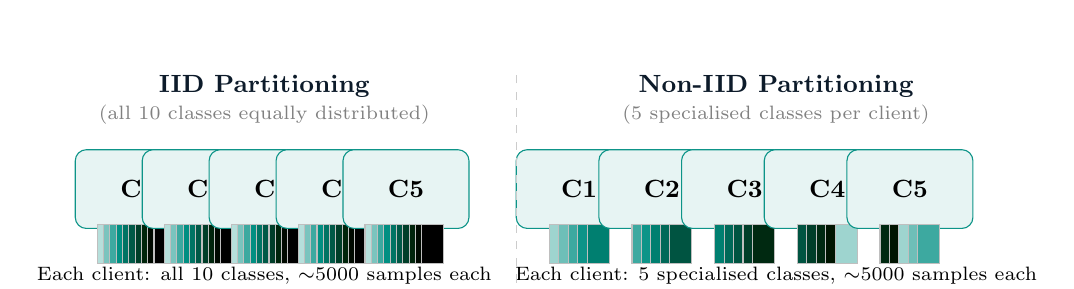
\begin{tikzpicture}[
  client/.style={rectangle, rounded corners=4pt, draw=tealcolor, fill=tealcolor!10,
                 minimum width=1.6cm, minimum height=1.0cm, font=\small\bfseries},
  classbox/.style={rectangle, draw=gray!50, fill=#1, minimum width=0.28cm,
                   minimum height=0.5cm, inner sep=0},
  label/.style={font=\small\bfseries, text=navycolor}
]

% IID side
\node[label] at (2.0, 3.5) {IID Partitioning};
\node[font=\scriptsize, text=gray] at (2.0, 3.15) {(all 10 classes equally distributed)};

\foreach \i/\name in {0/C1, 1/C2, 2/C3, 3/C4, 4/C5} {
  \node[client] (iid\i) at (\i*0.85+0.4, 2.2) {\name};
  % 10 small coloured class boxes per client
  \foreach \j in {0,...,9} {
    \pgfmathsetmacro\colval{int(mod(\j,10)*25+30)}
    \node[classbox=tealcolor!\colval] at (\i*0.85+0.08*\j+0.02, 1.5) {};
  }
}
\node[font=\scriptsize] at (2.0, 1.1) {Each client: all 10 classes, $\sim$5000 samples each};

% Non-IID side
\node[label] at (8.5, 3.5) {Non-IID Partitioning};
\node[font=\scriptsize, text=gray] at (8.5, 3.15) {(5 specialised classes per client)};

\foreach \i/\name/\startcol in {0/C1/0, 1/C2/2, 2/C3/4, 3/C4/6, 4/C5/8} {
  \node[client] (ni\i) at (\i*1.05+6.0, 2.2) {\name};
  \foreach \j in {0,...,4} {
    \pgfmathsetmacro\colidx{int(mod(\startcol+\j,10))}
    \pgfmathsetmacro\colval{int(\colidx*20+40)}
    \node[classbox=tealcolor!\colval] at (\i*1.05+6.0+0.12*\j-0.24, 1.5) {};
  }
}
\node[font=\scriptsize] at (8.5, 1.1) {Each client: 5 specialised classes, $\sim$5000 samples each};

% Dividing line
\draw[gray!40, dashed] (5.2, 0.8) -- (5.2, 3.7);

\end{tikzpicture}
\caption{Comparison of IID and Non-IID partitioning for CIFAR-10 across 5 clients.
Under IID (left), each client receives a balanced sample of all 10 classes. Under
Non-IID (right), each client is assigned only 5 classes, creating specialised local
distributions. The colour of each small block represents a different class. This
specialisation is the mechanism by which Non-IID partitioning amplifies membership
leakage in the experiments of RQ4 and RQ6.}
\label{fig:noniid_diagram}
\end{figure}

\section{Confidence Score Distributions and EDA Insights}

A critical component of the exploratory analysis is the examination of the trained
model's output confidence distributions for member and non-member samples, because
these distributions are precisely what the membership attacker exploits. After
completing federated training, the global model was queried on 5,000 member samples
(drawn from the training set) and 5,000 non-member samples (drawn from the test
set).

On CIFAR-10, member samples showed a slightly higher mean maximum confidence
compared to non-member samples, but the distributions overlapped substantially.
This substantial overlap is the reason why the logistic regression attacker, which
operates on the full softmax confidence vector, achieved near-random AUC: the
confidence vectors for members and non-members are not linearly separable. However,
when the cross-entropy loss is examined as a single scalar feature rather than the
full vector, a clearer separation emerges. Member samples produce lower average loss
than non-members, because the model has been optimised to predict them correctly.
This separation is what the loss-based attack exploits.

On CIFAR-100, the same pattern was observed but with a more pronounced loss
separation. The harder classification task means the model fails more often on
non-members, producing substantially higher prediction loss, while the training
samples benefit from the model's direct optimisation on their specific labels.
The larger loss gap between members and non-members on CIFAR-100 directly explains
the higher loss-based attack AUC of 0.618 compared to 0.577 on CIFAR-10.

% ══════════════════════════════════════════════════════════════════════════════
\chapter{Method Description}

This study employs a unified experimental framework that simulates a federated
learning environment and systematically evaluates membership inference attacks
across three attacker capability tiers. The complete pipeline spans seven stages:
dataset preparation and partitioning, federated learning simulation, baseline
black-box attack evaluation, differential privacy defence, shadow model attack,
white-box gradient attack, and comparative evaluation across all methods. All
experiments were implemented in Python using TensorFlow 2.19.0 and executed on
Google Colab with a T4 GPU.

\section{Attacker Threat Model}

Before describing the specific attack implementations, it is important to formally
define the three attacker threat models evaluated in this study. The threat model
specifies what the attacker knows and what capabilities they possess.

\subsection{Tier 1: Black-Box Attacker (Controlled Baseline)}

The black-box attacker has \textit{query access only} to the trained global model.
Given an input sample $x$, the attacker can observe the model's output softmax
probability vector $f(x) \in [0,1]^C$. The attacker has no access to model
weights, gradients, or any training data. In the controlled baseline evaluation
(RQ1--RQ3), the attacker is also assumed to have access to labelled member and
non-member samples from the target dataset for training the attack classifier.
This assumption is unrealistic in the FL setting because training data never leaves
client devices, but it provides a useful upper bound on what a classifier attacker
can achieve with perfect knowledge of which samples are members.

\subsection{Tier 2: Realistic Shadow Model Attacker}

The shadow model attacker has \textit{query access only} to the target model but,
critically, does \textit{not} have access to any real training data from the target
FL system. Instead, the attacker possesses a dataset from a similar domain ---
in this study, CIFAR-100 images when attacking a CIFAR-10 target. The attacker
trains their own shadow federated model on this similar data, uses the known
membership labels of the shadow training to build an attack classifier, and then
transfers the classifier to the target model. This is the realistic black-box
threat model for federated learning, because it respects the constraint that
training data never leaves the client devices.

\subsection{Tier 3: White-Box Attacker}

The white-box attacker has \textit{full access to model weights and gradients}.
This corresponds to a compromised aggregation server that receives the global
model weights and can compute per-sample gradients using TensorFlow's
\texttt{GradientTape}. The white-box attacker represents the theoretical upper
bound on what an attacker with server-level access can achieve, and provides the
strongest possible membership signal through gradient norm features.

Figure~\ref{fig:threat_model} illustrates the three threat model tiers.

\begin{figure}[H]
\centering
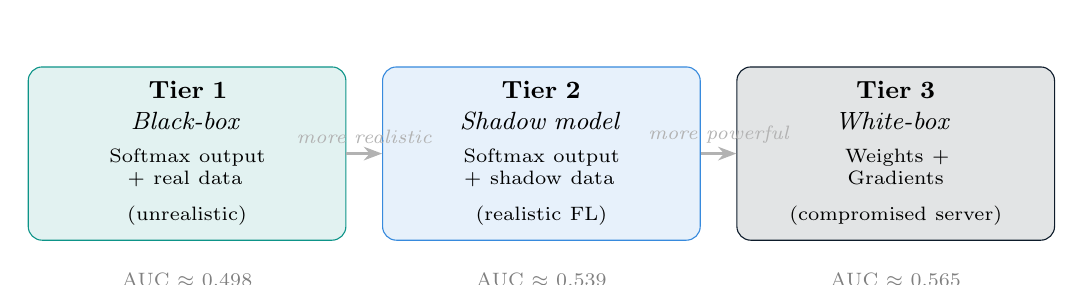
\begin{tikzpicture}[
  box/.style={rectangle, rounded corners=5pt, draw=#1, fill=#1!12,
              text width=3.8cm, minimum height=2.2cm, align=center,
              font=\small},
  arrow/.style={-Stealth, thick, color=gray!60},
  label/.style={font=\small\bfseries}
]

\node[box=tealcolor] (t1) at (0,0) {
  \textbf{Tier 1}\\
  \textit{Black-box}\\[4pt]
  \scriptsize Softmax output\\
  \scriptsize + real data\\[2pt]
  \scriptsize (unrealistic)
};

\node[box=bluecolor] (t2) at (4.5,0) {
  \textbf{Tier 2}\\
  \textit{Shadow model}\\[4pt]
  \scriptsize Softmax output\\
  \scriptsize + shadow data\\[2pt]
  \scriptsize (realistic FL)
};

\node[box=navycolor] (t3) at (9,0) {
  \textbf{Tier 3}\\
  \textit{White-box}\\[4pt]
  \scriptsize Weights +\\
  \scriptsize Gradients\\[2pt]
  \scriptsize (compromised server)
};

\draw[arrow] (t1) -- (t2) node[midway, above, font=\scriptsize\itshape] {more realistic};
\draw[arrow] (t2) -- (t3) node[midway, above, font=\scriptsize\itshape] {more powerful};

\node[font=\scriptsize, text=gray] at (0,-1.6) {AUC $\approx$ 0.498};
\node[font=\scriptsize, text=gray] at (4.5,-1.6) {AUC $\approx$ 0.539};
\node[font=\scriptsize, text=gray] at (9,-1.6) {AUC $\approx$ 0.565};

\end{tikzpicture}
\caption{Three-tier attacker capability hierarchy evaluated in this study (IID,
CIFAR-10). Tier 1 represents the controlled but unrealistic black-box attacker
who has access to real training data. Tier 2 is the realistic shadow model
attacker who uses only similar-domain data. Tier 3 is the white-box attacker
with full gradient access. AUC values shown are from the IID CIFAR-10 experiments.}
\label{fig:threat_model}
\end{figure}

\section{Data Partitioning}

\subsection{IID Partitioning}
The training data for each dataset was partitioned across federated clients using
IID partitioning. The full training set of 50,000 samples was first randomly
shuffled using a fixed random seed of 42, then divided into equal-sized subsets
using NumPy's \texttt{array\_split} function. Under this scheme, each client
receives a random and balanced sample from the full class distribution.

\subsection{Non-IID Partitioning}
For the Non-IID experiments, the class-based partitioning strategy described in
Section~\ref{sec:noniid_partitioning} was used. Client $i$ was assigned data
from classes $\{(i \cdot k + j) \bmod C \mid j = 0, \ldots, k-1\}$, where $C$
is the total number of classes and $k$ is the number of classes per client.

\section{Model Architecture}

Two CNN architectures were defined to address RQ3. The \textit{small} model
consists of two convolutional blocks, each containing a Conv2D layer with ReLU
activation and same padding, followed by MaxPooling2D. The first block uses 32
filters and the second 64 filters, both with $3 \times 3$ kernels. A Dense layer
of 128 units with ReLU activation and Dropout (rate 0.3) follows the flattened
convolutional output. The final layer is a softmax Dense layer with $C$ output
units. The \textit{large} model uses four convolutional layers in two blocks of
two (64 and 128 filters), a Dense layer of 256 units with Dropout (0.4), and the
same softmax output layer. Both models used the Adam optimiser at learning rate
0.001 and sparse categorical cross-entropy loss.

\section{Federated Learning Simulation}

Federated learning was simulated using the FedAvg algorithm. At each round, the
server broadcasts the global weights to all clients. Each client trains a local
copy for a fixed number of epochs and returns the updated weights. The server
aggregates using the weighted average:

\begin{equation}
  w_{t+1} = \sum_{k=1}^{K} \frac{n_k}{n} \, w_k^t
\end{equation}

\noindent where $K$ is the number of clients, $n_k$ is client $k$'s dataset size,
$n$ is the total sample count, and $w_k^t$ is the weight vector returned by
client $k$ at round $t$.

\begin{algorithm}[H]
\caption{Federated Averaging (FedAvg)}
\label{alg:fedavg}
\begin{algorithmic}[1]
\State \textbf{Input:} $K$ clients, $T$ rounds, $E$ local epochs, batch size $B$, learning rate $\eta$
\State \textbf{Output:} Global model weights $w_T$
\State Initialise global model weights $w_0$
\For{round $t = 1$ to $T$}
    \State Server broadcasts $w_{t-1}$ to all $K$ clients
    \For{each client $k = 1$ to $K$} \textbf{in parallel}
        \State Initialise local model with $w_{t-1}$
        \State Train locally for $E$ epochs with batch size $B$
        \State Return updated weights $w_k^t$ to server
    \EndFor
    \State $w_t \leftarrow \sum_{k=1}^{K} \frac{n_k}{n} \, w_k^t$ \Comment{Weighted average}
\EndFor
\State \Return $w_T$
\end{algorithmic}
\end{algorithm}

\begin{figure}[H]
  \centering
  \includegraphics[width=0.82\textwidth]{cifar10_convergence.png}
  \caption{FedAvg convergence on CIFAR-10 with 5 clients over 10 communication
  rounds (Notebook~01). Global test accuracy rises from 48.0\% at round~1 to
  72.0\% at round~10, demonstrating stable and consistent convergence under
  IID partitioning. The curve flattens after round~8, indicating the model has
  approached its capacity limit under this configuration.}
  \label{fig:cifar10_convergence}
\end{figure}

\noindent Figure~\ref{fig:fl_architecture} illustrates the FedAvg architecture
used throughout all experiments.

\begin{figure}[H]
\centering
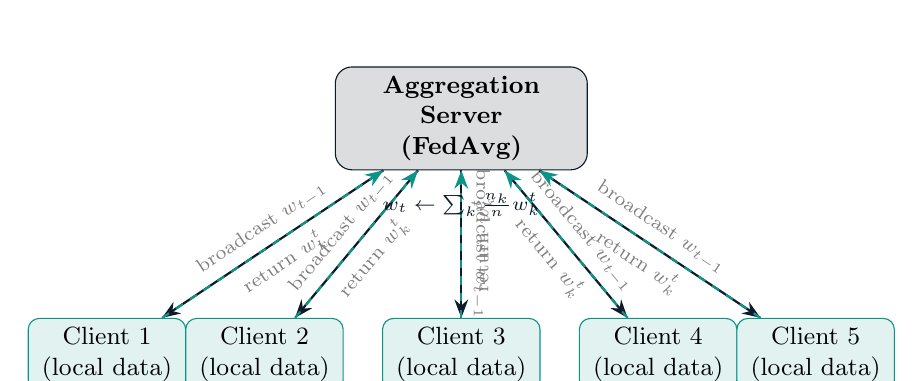
\begin{tikzpicture}[
  server/.style={rectangle, rounded corners=6pt, draw=navycolor, fill=navycolor!15,
                 minimum width=3.2cm, minimum height=1.2cm, align=center, font=\small\bfseries},
  client/.style={rectangle, rounded corners=4pt, draw=tealcolor, fill=tealcolor!12,
                 minimum width=2.0cm, minimum height=0.9cm, align=center, font=\small},
  arrow/.style={-Stealth, thick},
  label/.style={font=\scriptsize, text=gray}
]

\node[server] (server) at (5, 4.5) {Aggregation\\Server\\(FedAvg)};

\foreach \i/\x/\name in {1/0.5/Client 1, 2/2.5/Client 2, 3/5.0/Client 3, 4/7.5/Client 4, 5/9.5/Client 5} {
  \node[client] (c\i) at (\x, 1.5) {\name\\(local data)};
  \draw[arrow, color=navycolor] (server) -- (c\i)
    node[midway, sloped, label, above] {broadcast $w_{t-1}$};
  \draw[arrow, color=tealcolor, dashed] (c\i) -- (server)
    node[midway, sloped, label, below] {return $w_k^t$};
}

\node[font=\scriptsize, text=navycolor, align=center] at (5, 3.4)
  {$w_t \leftarrow \sum_{k} \frac{n_k}{n} w_k^t$};

\end{tikzpicture}
\caption{FedAvg federated learning architecture used in all experiments. The
central server broadcasts global weights to all clients at the start of each
round. Each client trains locally on their private data and returns updated
weights. The server computes a weighted average proportional to local dataset
size. Raw training data never leaves client devices.}
\label{fig:fl_architecture}
\end{figure}

\section{Baseline Black-Box Attack (RQ1--RQ5)}

The baseline black-box attack pipeline constructs an attacker dataset by querying
the trained global model on 5,000 member samples (from the training set) and
5,000 non-member samples (from the test set). The $C$-dimensional softmax output
vector for each sample forms the attack feature vector. A logistic regression
binary classifier is trained on 70\% of this dataset and evaluated on the
remaining 30\%.

\begin{algorithm}[H]
\caption{Black-Box Membership Inference Attack}
\label{alg:mia}
\begin{algorithmic}[1]
\State \textbf{Input:} Global model $f$, training set $X_{\text{train}}$, test set $X_{\text{test}}$, attack size $N$
\State \textbf{Output:} Attack metrics (AUC, Recall)
\State Sample $N$ members $X_m \subset X_{\text{train}}$ $\rightarrow$ label $1$
\State Sample $N$ non-members $X_{nm} \subset X_{\text{test}}$ $\rightarrow$ label $0$
\For{each sample $x \in X_m \cup X_{nm}$}
    \State Query $f(x)$ $\rightarrow$ softmax vector $\mathbf{p} \in [0,1]^C$
\EndFor
\State Build attacker dataset $X_{\text{atk}} = [\mathbf{p}_1, \ldots, \mathbf{p}_{2N}]$, $y_{\text{atk}} \in \{0,1\}^{2N}$
\State Split 70/30, train logistic regression, evaluate AUC and Recall
\State \Return AUC, Recall
\end{algorithmic}
\end{algorithm}

\section{Baseline Attack Methods}

Three additional baseline attack methods were evaluated. The \textit{random
baseline} assigns uniform random scores, providing the theoretical performance
floor at AUC 0.50. The \textit{threshold attack} uses $\max(\mathbf{p})$ as the
membership score, predicting membership when the model's highest confidence
exceeds 0.5. The \textit{loss-based attack} uses the negative cross-entropy loss:

\begin{equation}
  s_{\text{loss}}(x) = \sum_{c=1}^{C} \mathbf{1}[c = \hat{y}] \log p_c
  \quad \text{where } \hat{y} = \arg\max_c p_c
\end{equation}

\noindent Higher scores correspond to lower prediction loss, indicating higher
membership likelihood. The loss-based attack requires no training data, unlike the
logistic regression classifier.

\section{Differential Privacy Defence (RQ5)}
\label{sec:dpmethod}

DP-SGD was implemented from scratch using TensorFlow's \texttt{GradientTape} API.
The mechanism modifies the standard gradient update in two steps. First, each
per-sample gradient is clipped to L2 norm $\leq C$. Second, Gaussian noise is
added before the weight update:

\begin{equation}
  \tilde{g} = \frac{1}{B} \left( \sum_{i=1}^{B} \text{clip}(g_i, C)
  + \mathcal{N}(0, \sigma^2 C^2 \mathbf{I}) \right)
\end{equation}

Three configurations were evaluated with clipping bound $C = 1.0$: no DP
(baseline), moderate privacy ($\varepsilon = 10$, $\sigma = 1.1$), and strong
privacy ($\varepsilon = 1$, $\sigma = 3.0$). All DP experiments used CIFAR-10,
IID partitioning, 5 clients, 5 rounds, and 2 local epochs with SGD as the base
optimiser.

\section{Shadow Model Attack (RQ6)}

The shadow model attack addresses the realistic FL threat model where the attacker
cannot access real training data. The attack proceeds in five steps, illustrated
in Figure~\ref{fig:shadow_pipeline}.

\begin{figure}[H]
\centering
\begin{tikzpicture}[
  step/.style={rectangle, rounded corners=5pt, draw=tealcolor, fill=tealcolor!10,
               text width=2.2cm, minimum height=1.4cm, align=center, font=\scriptsize},
  arrow/.style={-Stealth, thick, color=navycolor},
  note/.style={font=\scriptsize\itshape, text=gray, align=center}
]

\node[step] (s1) at (0,0) {\textbf{Step 1}\\Shadow\\dataset\\(CIFAR-100)};
\node[step] (s2) at (2.8,0) {\textbf{Step 2}\\Train shadow\\FL model\\(FedAvg)};
\node[step] (s3) at (5.6,0) {\textbf{Step 3}\\Query shadow\\model\\(known labels)};
\node[step] (s4) at (8.4,0) {\textbf{Step 4}\\Train attack\\classifier\\(LR)};
\node[step] (s5) at (11.2,0) {\textbf{Step 5}\\Apply to\\target model\\(CIFAR-10)};

\draw[arrow] (s1) -- (s2);
\draw[arrow] (s2) -- (s3);
\draw[arrow] (s3) -- (s4);
\draw[arrow] (s4) -- (s5);

\node[note] at (0,-1.3)    {similar domain\\not the same};
\node[note] at (2.8,-1.3)  {attacker controls\\shadow FL};
\node[note] at (5.6,-1.3)  {shadow members\\\& non-members};
\node[note] at (8.4,-1.3)  {6-dim feature\\extraction};
\node[note] at (11.2,-1.3) {no real\\training data used};

\end{tikzpicture}
\caption{Shadow model attack pipeline (RQ6). The attacker uses CIFAR-100 as
shadow data --- same 32$\times$32 RGB format, completely different 100 classes.
A shadow federated model is trained on CIFAR-100 using FedAvg. Because the
attacker controls the shadow training, they know which samples are shadow members
and non-members. The attack classifier is trained on shadow model predictions and
then transferred to the real CIFAR-10 target. No CIFAR-10 training samples are
used at any point.}
\label{fig:shadow_pipeline}
\end{figure}

\noindent Because the shadow model (100 output classes) and the target model (10
output classes) produce softmax vectors of different dimensions, raw softmax
vectors cannot be directly compared. Instead, six architecture-agnostic features
are extracted:

\begin{itemize}[leftmargin=1.5em, itemsep=2pt]
  \item \textbf{Max confidence:} $\max_c p_c$ --- highest predicted class probability
  \item \textbf{Prediction entropy:} $-\sum_c p_c \log p_c$ --- uncertainty of the distribution
  \item \textbf{Top-3 confidence values:} the three largest softmax values, capturing confidence spread
  \item \textbf{Loss proxy:} $-\log(\max_c p_c)$ --- approximation of cross-entropy loss
\end{itemize}

These six features are computed identically from any softmax output regardless
of the number of output classes, enabling the attack classifier trained on shadow
model (100-class) outputs to be applied to the target model (10-class) outputs.

\begin{algorithm}[H]
\caption{Shadow Model Membership Inference Attack}
\label{alg:shadow}
\begin{algorithmic}[1]
\State \textbf{Input:} Target model $f_T$ (CIFAR-10), shadow dataset $D_S$ (CIFAR-100), attack size $N$
\State \textbf{Output:} Attack metrics on target model
\State Train shadow FL model $f_S$ on $D_S$ using FedAvg
\State Sample $N$ shadow members $X_{Sm}$ (trained on by $f_S$) $\rightarrow$ label $1$
\State Sample $N$ shadow non-members $X_{Snm}$ (not trained on) $\rightarrow$ label $0$
\For{each sample $x \in X_{Sm} \cup X_{Snm}$}
    \State Query $f_S(x)$ $\rightarrow$ extract 6 features $\phi(f_S(x))$
\EndFor
\State Train attack classifier $g$ on $\{(\phi(f_S(x)), y)\}$
\For{each target sample $x \in X_{Tm} \cup X_{Tnm}$}
    \State Query $f_T(x)$ $\rightarrow$ extract 6 features $\phi(f_T(x))$
\EndFor
\State Evaluate $g$ on $\{\phi(f_T(x))\}$ $\rightarrow$ compute AUC, Recall
\State \Return AUC, Recall
\end{algorithmic}
\end{algorithm}

\section{White-Box Attack (RQ7)}

The white-box attack is implemented following Nasr et al.~\cite{nasr2019comprehensive}.
For each sample, TensorFlow's \texttt{GradientTape} is used to compute the
gradient of the cross-entropy loss with respect to all trainable weight matrices.
The per-layer gradient L2 norms are extracted as membership features.

\begin{equation}
  \nabla_{w_\ell} \mathcal{L}(f(x), y) \quad \text{for each layer } \ell = 1, \ldots, L
\end{equation}

The intuition is straightforward: a model produces small gradients on samples it
has already learned (members) and large gradients on samples it has not seen
(non-members). This gradient magnitude difference is a direct consequence of the
model's convergence on training data. The feature vector for each sample is:

\begin{equation}
  \phi_{\text{WB}}(x) = \left[ \|\nabla_{w_1}\mathcal{L}\|_2,\,
  \ldots,\, \|\nabla_{w_L}\mathcal{L}\|_2,\,
  \|\nabla_{w_L}\mathcal{L}\|_2,\,
  \mathcal{L}(f(x),y),\, \max_c p_c,\, H(\mathbf{p}) \right]
\end{equation}

\noindent where $H(\mathbf{p}) = -\sum_c p_c \log p_c$ is the prediction entropy.
Feature scaling via StandardScaler is applied before logistic regression training.

\begin{algorithm}[H]
\caption{White-Box Gradient Membership Inference Attack}
\label{alg:whitebox}
\begin{algorithmic}[1]
\State \textbf{Input:} Global model $f$ with weights $\{w_\ell\}$, samples $X_m$, $X_{nm}$
\State \textbf{Output:} Attack AUC, Recall
\For{each sample $x \in X_m \cup X_{nm}$}
    \State Compute $\nabla_{w_\ell} \mathcal{L}(f(x), y)$ for all $\ell$ using \texttt{GradientTape}
    \State Extract $\phi_{\text{WB}}(x)$: per-layer gradient norms + loss + confidence + entropy
\EndFor
\State Scale features, split 70/30, train logistic regression classifier
\State Evaluate on test split $\rightarrow$ compute AUC and Recall
\State \Return AUC, Recall
\end{algorithmic}
\end{algorithm}

\section{Experimental Design Summary}

Table~\ref{tab:exp_design} summarises the complete experimental design across all
seven research questions and seven notebooks.

\begin{table}[H]
  \centering
  \caption{Complete experimental design across all research questions.}
  \label{tab:exp_design}
  \begin{tabular}{lllll}
    \toprule
    \textbf{RQ} & \textbf{Notebook} & \textbf{Dataset} & \textbf{Attack} & \textbf{Key variable} \\
    \midrule
    RQ1 & 01, 02 & C-10, C-100 & BB + Loss & Baseline IID \\
    RQ2 & 01, 02 & C-10, C-100 & BB + Loss & Clients: 2, 5, 10 \\
    RQ3 & 01, 02 & C-10, C-100 & BB + Loss & Model: small, large \\
    RQ4 & 03a, 03b & C-10, C-100 & BB + Loss & IID vs Non-IID \\
    RQ5 & 04 & C-10 & Loss + LR & $\varepsilon$: $\infty$, 10, 1 \\
    RQ6 & 05 & C-10 (shadow: C-100) & Shadow model & Realistic attacker \\
    RQ7 & 06 & C-10 & White-box gradient & Gradient access \\
    \bottomrule
  \end{tabular}
\end{table}

\section{Evaluation Metrics}

All attacks were evaluated using four metrics: \textit{accuracy}, \textit{precision},
\textit{recall}, and \textit{AUC} (Area Under the ROC Curve). For a balanced
attacker dataset, all metrics have a random-chance baseline of 0.50. AUC is the
primary metric because it measures the attacker's ability to rank members above
non-members across all decision thresholds, independent of the specific threshold
chosen. Recall is reported as a secondary metric because it captures the proportion
of actual training members correctly identified by the attacker, which is the most
practically meaningful privacy violation.

% ══════════════════════════════════════════════════════════════════════════════
\chapter{Experiments, Results, and Evaluation}

\section{Experimental Setup}

All experiments were conducted on Google Colab using a T4 GPU with TensorFlow
2.19.0 and a fixed random seed of 42. The seven notebooks are self-contained and
fully reproducible. The attacker dataset for RQ1--RQ4 consisted of 5,000 member
and 5,000 non-member samples; for RQ2 and RQ3 experiment loops, reduced samples
of 1,000 per group were used to manage RAM constraints on the free Colab tier.
The shadow model attack (RQ6) used 5,000 shadow members and non-members from
CIFAR-100 and evaluated on 5,000 target members and non-members from CIFAR-10.
The white-box attack (RQ7) used 2,000 members and non-members due to the
computational cost of per-sample gradient computation.

\section{Baseline Attack Comparison (RQ1)}

Table~\ref{tab:baseline} presents the baseline comparison for CIFAR-10 and
CIFAR-100 under the base federated configuration.

\begin{table}[H]
  \centering
  \caption{Baseline attack comparison --- CIFAR-10 and CIFAR-100 (RQ1, IID, 5 clients, 10 rounds).}
  \label{tab:baseline}
  \begin{tabular}{lcccc}
    \toprule
    \textbf{Method} & \textbf{C-10 Acc.} & \textbf{C-10 AUC} & \textbf{C-100 Acc.} & \textbf{C-100 AUC} \\
    \midrule
    Random baseline                    & 0.4925 & 0.4969 & 0.4925 & 0.4969 \\
    Threshold attack                   & 0.5128 & 0.5355 & 0.5349 & 0.5408 \\
    Loss-based attack                  & 0.5506 & 0.5768 & 0.5874 & 0.6180 \\
    Logistic regression (trained)      & 0.4940 & 0.4967 & 0.5177 & 0.5162 \\
    \bottomrule
  \end{tabular}
\end{table}

On CIFAR-10, all four methods produced AUC values near 0.50. The loss-based
attack achieved the highest AUC of 0.577, followed by the threshold attack at
0.536. The logistic regression attacker achieved 0.497, below even random chance,
indicating that FedAvg's weight averaging has destroyed the structured patterns
in the confidence vector that a linear classifier would need. This is a direct
empirical confirmation of the FedAvg privacy mechanism: individual client
memorisation signals are diluted through weighted averaging to the point where
a linear classifier operating on the full softmax vector finds nothing useful.

However, the loss-based attack's AUC of 0.577 reveals that the membership signal
has not been completely eliminated --- it has merely changed form. Rather than
residing in the full confidence vector pattern, it is concentrated in a single
scalar value: the cross-entropy loss on the predicted class. This scalar survives
the averaging process because it is a direct consequence of how well the global
model has learned to predict the sample correctly. Members, which were used in
training, produce systematically lower loss than non-members.

On CIFAR-100, the same ordering was observed with stronger signals overall. The
loss-based attack achieved AUC of 0.618 --- the highest across all IID
experiments. This confirms the dataset complexity hypothesis: harder classification
tasks produce larger generalisation gaps, which manifest as larger loss differences
between members and non-members, which in turn make the loss-based attack more
discriminative.

\textbf{Key finding (RQ1):} The primary membership vulnerability in FedAvg-trained
models is the prediction loss signal, not the confidence vector pattern. FedAvg
resists classifier-based attacks but not loss-based attacks.

\begin{figure}[H]
  \centering
  \begin{subfigure}[t]{0.48\textwidth}
    \centering
    \includegraphics[width=\textwidth]{cifar10_rq1_results.png}
    \caption{CIFAR-10: LR attacker AUC = 0.4973, Recall = 0.3580. Both sit
    below random chance, confirming the logistic regression classifier finds
    no useful structure in the averaged softmax confidence vectors.}
    \label{fig:cifar10_rq1_bar}
  \end{subfigure}
  \hfill
  \begin{subfigure}[t]{0.48\textwidth}
    \centering
    \includegraphics[width=\textwidth]{cifar100_rq1_results.png}
    \caption{CIFAR-100: LR attacker AUC = 0.5071, Recall = 0.4667. Slightly
    above random chance, reflecting marginally richer patterns from the harder
    100-class task. Loss-based AUC reaches 0.618.}
    \label{fig:cifar100_rq1_bar}
  \end{subfigure}
  \caption{RQ1 black-box MIA results for the logistic regression attacker on
  CIFAR-10 (left) and CIFAR-100 (right). The dashed line marks the 0.50 random
  chance baseline. Both datasets show near-random AUC for the LR classifier,
  while the loss-based attack achieves 0.577 and 0.618 respectively
  (Table~\ref{tab:baseline}).}
  \label{fig:rq1_bars}
\end{figure}

\begin{figure}[H]
  \centering
  \includegraphics[width=0.75\textwidth]{cifar10_rq1_roc_comparison.png}
  \caption{ROC curves for CIFAR-10 (RQ1) comparing the logistic regression
  attacker (LR, AUC = 0.497, solid blue) and the loss-based attack (AUC = 0.538,
  dashed green) against the random chance diagonal. The LR curve hugs the
  diagonal throughout, confirming near-zero discriminative power. The loss-based
  curve separates consistently above the diagonal in the 0.2--0.8 FPR range,
  visualising the partial membership leakage through prediction loss.}
  \label{fig:cifar10_roc}
\end{figure}

\section{RQ2 --- Effect of Number of Clients}

Table~\ref{tab:rq2} presents attack AUC across different federation sizes.

\begin{table}[H]
  \centering
  \caption{RQ2 results --- attack AUC vs.\ number of clients (IID, loss-based attack).}
  \label{tab:rq2}
  \begin{tabular}{ccccc}
    \toprule
    \textbf{Clients} & \textbf{C-10 Global Acc.} & \textbf{C-10 AUC} & \textbf{C-100 Global Acc.} & \textbf{C-100 AUC} \\
    \midrule
    2  & 0.7069 & 0.4932 & 0.3819 & 0.4782 \\
    5  & 0.6784 & 0.5123 & 0.3270 & 0.4888 \\
    10 & 0.6415 & 0.5027 & 0.2746 & 0.4988 \\
    \bottomrule
  \end{tabular}
\end{table}

Across both datasets, attack AUC showed negligible and inconsistent variation
with the number of clients. On CIFAR-10, AUC fluctuated between 0.493 and 0.512
with no monotonic trend. On CIFAR-100, AUC increased slightly from 0.478 at
2 clients to 0.499 at 10 clients, but remained entirely below random chance.
Neither direction is practically meaningful.

The absence of a consistent client count effect is theoretically explained by
the FedAvg aggregation mechanism. Because weights are averaged proportionally to
dataset size, adding more clients with equal-sized datasets does not fundamentally
change the averaging dynamics --- the global model still converges to the same
point on the loss landscape. From an information-theoretic perspective, the
membership signal per sample depends on how much the global model has overfit to
that sample, which is determined by the learning dynamics of FedAvg rather than
by the number of participants.

\textbf{Key finding (RQ2):} The number of federated clients has no meaningful or
consistent effect on black-box MIA success under IID conditions. FedAvg provides
equivalent privacy regardless of federation size within the evaluated range.

\begin{figure}[H]
  \centering
  \begin{subfigure}[t]{0.48\textwidth}
    \centering
    \includegraphics[width=\textwidth]{cifar10_rq2_clients.png}
    \caption{CIFAR-10: Attack AUC fluctuates between 0.499--0.525 with no
    monotonic trend across 2, 5, and 10 clients. All values remain near the
    0.50 random chance line.}
    \label{fig:cifar10_rq2}
  \end{subfigure}
  \hfill
  \begin{subfigure}[t]{0.48\textwidth}
    \centering
    \includegraphics[width=\textwidth]{cifar100_rq2_clients.png}
    \caption{CIFAR-100: Attack AUC ranges 0.473--0.482, all below random
    chance. The slight upward trend is negligible and not practically
    meaningful.}
    \label{fig:cifar100_rq2}
  \end{subfigure}
  \caption{RQ2 results --- effect of number of federated clients on black-box
  MIA success for CIFAR-10 (left) and CIFAR-100 (right). Neither dataset shows
  a meaningful relationship between client count and attack AUC.}
  \label{fig:rq2_clients}
\end{figure}

\section{RQ3 --- Effect of Model Complexity}

Table~\ref{tab:rq3} presents attack results for the two CNN architectures.

\begin{table}[H]
  \centering
  \caption{RQ3 results --- attack AUC vs.\ model complexity (IID, 5 clients).}
  \label{tab:rq3}
  \begin{tabular}{lcccc}
    \toprule
    \textbf{Model} & \textbf{C-10 Global Acc.} & \textbf{C-10 AUC} & \textbf{C-100 Global Acc.} & \textbf{C-100 AUC} \\
    \midrule
    Small CNN ($\sim$200K params) & 0.6811 & 0.4946 & 0.3304 & 0.5195 \\
    Large CNN ($\sim$1.2M params) & 0.7442 & 0.5031 & 0.3642 & 0.4867 \\
    \bottomrule
  \end{tabular}
\end{table}

On CIFAR-10, both model sizes produced AUC near 0.50 with only a marginal
difference of 0.009. On CIFAR-100, the pattern reversed: the small model showed
slightly higher AUC (0.520) than the large model (0.487). This reversal is
inconsistent with the hypothesis that larger models overfit more and are therefore
more vulnerable. Instead, it suggests that in the federated setting, model
complexity does not reliably control privacy leakage when weight averaging is
applied. The large model's higher classification accuracy (74.42\% vs 68.11\% on
CIFAR-10) does not translate into higher membership distinguishability at the
softmax output level, because the averaging process has suppressed memorisation
signals regardless of model capacity.

\textbf{Key finding (RQ3):} Model complexity does not reliably affect black-box
MIA success under FedAvg. Both small and large models show near-random AUC,
confirming that the averaging mechanism is the dominant factor rather than
individual model capacity.

\begin{figure}[H]
  \centering
  \begin{subfigure}[t]{0.48\textwidth}
    \centering
    \includegraphics[width=\textwidth]{cifar10_rq3_complexity.png}
    \caption{CIFAR-10: Small CNN (AUC = 0.495) vs.\ Large CNN (AUC = 0.512).
    The 0.017 difference is not practically meaningful. Recall is lower for
    the Large CNN (0.360 vs 0.457), suggesting larger models produce more
    uniform confidence outputs after FedAvg averaging.}
    \label{fig:cifar10_rq3}
  \end{subfigure}
  \hfill
  \begin{subfigure}[t]{0.48\textwidth}
    \centering
    \includegraphics[width=\textwidth]{cifar100_rq3_complexity.png}
    \caption{CIFAR-100: Small CNN (AUC = 0.485) vs.\ Large CNN (AUC = 0.486).
    Essentially zero difference, confirming model complexity has no predictive
    value for black-box MIA success under FedAvg.}
    \label{fig:cifar100_rq3}
  \end{subfigure}
  \caption{RQ3 results --- model complexity vs.\ black-box MIA success for
  CIFAR-10 (left) and CIFAR-100 (right). FedAvg weight averaging is the dominant
  privacy mechanism regardless of architecture capacity.}
  \label{fig:rq3_complexity}
\end{figure}

\section{Dataset Complexity Comparison}

Table~\ref{tab:dataset_comparison} provides a direct comparison of attack
performance across both datasets, highlighting the effect of classification
difficulty on privacy leakage.

\begin{table}[H]
  \centering
  \caption{Direct comparison of attack performance across datasets (RQ1, IID, 5 clients).}
  \label{tab:dataset_comparison}
  \begin{tabular}{lccc}
    \toprule
    \textbf{Metric} & \textbf{CIFAR-10} & \textbf{CIFAR-100} & \textbf{Baseline} \\
    \midrule
    Accuracy          & 0.4940 & 0.5177 & 0.50 \\
    Precision         & 0.4929 & 0.5189 & 0.50 \\
    Recall            & 0.4160 & 0.4840 & 0.50 \\
    AUC (Log.\ Reg.)  & 0.4967 & 0.5162 & 0.50 \\
    AUC (Loss-based)  & 0.5768 & 0.6180 & 0.50 \\
    Global Model Acc. & 0.7160 & 0.3759 & ---  \\
    \bottomrule
  \end{tabular}
\end{table}

The 0.041 difference in loss-based AUC between CIFAR-10 and CIFAR-100 confirms
that dataset complexity amplifies the loss-based membership signal. The lower
global accuracy on CIFAR-100 (37.59\%) compared to CIFAR-10 (71.60\%) means the
model generalises poorly on CIFAR-100, producing substantially higher prediction
loss on non-members. This widens the loss gap between members (who benefit from
direct optimisation) and non-members (who do not), making the membership signal
more discriminative.

\section{Non-IID Extension (RQ4)}

\subsection{CIFAR-10: IID vs.\ Non-IID}

\begin{table}[H]
  \centering
  \caption{CIFAR-10 --- IID vs.\ Non-IID comparison (5 clients, 5 classes per client).}
  \label{tab:noniid_cifar10}
  \begin{tabular}{lcccc}
    \toprule
    \textbf{Condition} & \textbf{Global Acc.} & \textbf{LR AUC} & \textbf{Loss AUC} & \textbf{Leakage} \\
    \midrule
    IID             & 0.7160 & 0.4831 & 0.5401 & Low \\
    Non-IID (5/10)  & 0.4931 & 0.4981 & 0.5644 & Moderate \\
    \midrule
    \textit{Change} & $-0.223$ & $+0.015$ & $\mathbf{+0.024}$ & Increased \\
    \bottomrule
  \end{tabular}
\end{table}

The Non-IID condition produced a meaningful increase in loss-based AUC of +0.024.
The mechanism behind this increase is the following. When clients receive only
5 out of 10 classes, their local models develop strong overconfidence on their
assigned classes through repeated local optimisation on a narrow class distribution.
When these specialised local models are aggregated through FedAvg, the resulting
global model retains traces of this specialisation: it is systematically more
confident and incurs lower loss on samples from the classes that dominated each
client's local training. This differential confidence partially survives the
averaging process, widening the loss gap between members and non-members and
making the loss-based attack more effective.

The global model accuracy drop from 71.60\% to 49.31\% under Non-IID confirms
the well-known convergence degradation of FedAvg under heterogeneous data: when
client gradients point in conflicting directions, the averaged update moves the
global model towards a suboptimal compromise. Importantly, this accuracy degradation
and the increased privacy leakage are causally linked --- both arise from the same
underlying phenomenon of client specialisation.

\begin{figure}[H]
  \centering
  \includegraphics[width=0.85\textwidth]{cifar10_noniid_convergence.png}
  \caption{FedAvg convergence curves for CIFAR-10 under IID (blue) and Non-IID
  (orange) partitioning over 10 rounds. The IID model converges smoothly to
  71.60\%, while Non-IID reaches only 49.31\% due to conflicting gradient
  directions from client specialisation. This accuracy gap is causally linked
  to the +0.024 increase in loss-based attack AUC.}
  \label{fig:cifar10_noniid_convergence}
\end{figure}

\begin{figure}[H]
  \centering
  \includegraphics[width=\textwidth]{cifar10_noniid_comparison.png}
  \caption{IID vs.\ Non-IID comparison on CIFAR-10 (RQ4). \textbf{Left:}
  Attack AUC showing that Non-IID loss-based AUC (0.566) exceeds IID (0.541)
  by +0.024. LR AUC shows a smaller increase (+0.034). \textbf{Right:}
  Overlaid ROC curves confirming Non-IID (orange) sits above IID (blue) across
  all FPR thresholds.}
  \label{fig:cifar10_noniid}
\end{figure}

\subsection{CIFAR-100: IID vs.\ Non-IID}

\begin{table}[H]
  \centering
  \caption{CIFAR-100 --- IID vs.\ Non-IID comparison (5 clients, 50 classes per client).}
  \label{tab:noniid_cifar100}
  \begin{tabular}{lcccc}
    \toprule
    \textbf{Condition} & \textbf{Global Acc.} & \textbf{LR AUC} & \textbf{Loss AUC} & \textbf{Leakage} \\
    \midrule
    IID              & 0.3759 & 0.5407 & 0.5606 & Low \\
    Non-IID (50/100) & 0.2496 & 0.5426 & 0.5636 & Low \\
    \midrule
    \textit{Change}  & $-0.126$ & $+0.002$ & $+0.003$ & Negligible \\
    \bottomrule
  \end{tabular}
\end{table}

The negligible +0.003 increase on CIFAR-100 confirms that the degree of
heterogeneity is the critical variable, not merely the presence of Non-IID
conditions. Assigning 50 out of 100 classes per client produces mild
specialisation --- each client still sees a diverse range of categories and its
local model cannot develop strong class-specific overconfidence. This finding
has important implications: real-world FL systems need to be evaluated at their
actual degree of heterogeneity, not simply categorised as IID or Non-IID.

\begin{figure}[H]
  \centering
  \includegraphics[width=0.85\textwidth]{cifar100_noniid_convergence.png}
  \caption{FedAvg convergence for CIFAR-100 under IID and Non-IID over 10 rounds.
  Both curves show slower convergence than CIFAR-10. Non-IID reaches 24.96\% vs
  37.59\% for IID, but the smaller accuracy gap compared to CIFAR-10 reflects
  the lower heterogeneity at 50/100 classes per client.}
  \label{fig:cifar100_noniid_convergence}
\end{figure}

\begin{figure}[H]
  \centering
  \includegraphics[width=\textwidth]{cifar100_noniid_comparison.png}
  \caption{IID vs.\ Non-IID comparison on CIFAR-100 (RQ4). Both the bar chart
  (left) and ROC curves (right) confirm near-identical attack performance under
  both conditions, consistent with the low heterogeneity at 50/100 classes per
  client.}
  \label{fig:cifar100_noniid}
\end{figure}

\subsection{Summary of Non-IID Findings}

\begin{table}[H]
  \centering
  \caption{Complete summary of Non-IID vs.\ IID attack results across both datasets.}
  \label{tab:noniid_summary}
  \begin{tabular}{llcccl}
    \toprule
    \textbf{Dataset} & \textbf{Condition} & \textbf{Global Acc.} & \textbf{LR AUC} & \textbf{Loss AUC} & \textbf{Heterogeneity} \\
    \midrule
    CIFAR-10  & IID            & 0.7160 & 0.4831 & 0.5401          & None \\
    CIFAR-10  & Non-IID (5/10) & 0.4931 & 0.4981 & \textbf{0.5644} & Moderate \\
    CIFAR-100 & IID            & 0.3759 & 0.5407 & 0.5606          & None \\
    CIFAR-100 & Non-IID (50/100) & 0.2496 & 0.5426 & 0.5636        & Low \\
    \bottomrule
  \end{tabular}
\end{table}

\section{Differential Privacy Defence (RQ5)}

Table~\ref{tab:dp_results} presents the DP-SGD evaluation results.

\begin{table}[H]
  \centering
  \caption{DP-SGD defence results --- CIFAR-10, IID, 5 clients, 5 rounds (RQ5).}
  \label{tab:dp_results}
  \begin{tabular}{lcccc}
    \toprule
    \textbf{Configuration} & \textbf{$\varepsilon$} & \textbf{Global Acc.} & \textbf{Loss AUC} & \textbf{LR AUC} \\
    \midrule
    No DP (baseline)    & $\infty$ & 0.5300 & 0.5110 & 0.4750 \\
    Moderate DP         & 10       & 0.1210 & 0.4650 & 0.4620 \\
    Strong DP           & 1        & 0.1700 & 0.4980 & 0.5030 \\
    \midrule
    Random chance       & ---      & ---    & 0.5000 & 0.5000 \\
    \bottomrule
  \end{tabular}
\end{table}

The no-DP baseline achieves 53.0\% accuracy using a shorter 5-round SGD schedule.
At $\varepsilon = 10$ (moderate privacy), both attacks are suppressed below random
chance --- loss-based AUC drops to 0.465 and LR AUC to 0.462 --- but global
accuracy collapses to 12.1\%, rendering the model practically useless. At
$\varepsilon = 1$ (strong privacy), accuracy partially recovers to 17.0\% while
both attack AUCs remain near random chance (0.498 and 0.503). The non-monotone
relationship between $\varepsilon$ and accuracy ($\varepsilon = 1$ is worse for
privacy but better for accuracy than $\varepsilon = 10$) indicates that the noise
multiplier values interact with the SGD optimiser in a complex, non-linear way.

\textbf{Key finding (RQ5):} DP-SGD directly suppresses the loss-based membership
signal by reducing the loss gap between members and non-members. However, the
privacy-utility tradeoff under the evaluated configurations is not practically
viable, and further hyperparameter tuning is required to find a useful operating
point.

\begin{figure}[H]
  \centering
  \includegraphics[width=\textwidth]{dp_privacy_utility_tradeoff.png}
  \caption{Privacy-utility tradeoff bar chart for DP-SGD on CIFAR-10 (RQ5).
  Each group shows Global Accuracy (dark), Loss-Based AUC (teal), and LR AUC
  (blue) for No~DP, $\varepsilon=10$, and $\varepsilon=1$. Both attack AUCs
  fall to or below random chance under DP, while accuracy drops severely from
  53.0\% to 12.1\% ($\varepsilon=10$) and 17.0\% ($\varepsilon=1$).}
  \label{fig:dp_tradeoff_bar}
\end{figure}

\begin{figure}[H]
  \centering
  \begin{subfigure}[t]{0.48\textwidth}
    \centering
    \includegraphics[width=\textwidth]{dp_roc_curves.png}
    \caption{ROC curves under three DP configurations. No~DP (black, AUC =
    0.511) sits highest. $\varepsilon=10$ (orange, AUC = 0.465) dips below
    the diagonal, indicating the noise disrupts the membership signal. $\varepsilon=1$
    (red, AUC = 0.498) returns near-diagonal.}
    \label{fig:dp_roc}
  \end{subfigure}
  \hfill
  \begin{subfigure}[t]{0.48\textwidth}
    \centering
    \includegraphics[width=\textwidth]{dp_tradeoff_curve.png}
    \caption{Dual-axis tradeoff curve showing accuracy (black, left) and
    loss-based AUC (teal dashed, right) across epsilon. Both attack suppression
    and accuracy are non-monotone in $\varepsilon$, reflecting the complex
    interaction of noise with the SGD optimiser.}
    \label{fig:dp_tradeoff_line}
  \end{subfigure}
  \caption{DP-SGD defence evaluation (RQ5). Left: ROC curves showing attack
  suppression across epsilon. Right: dual-axis tradeoff curve directly
  illustrating the cost of privacy in this configuration.}
  \label{fig:dp_combined}
\end{figure}

\section{Shadow Model Attack (RQ6)}

\subsection{IID Results}

Table~\ref{tab:shadow_iid} presents the complete shadow model attack results
under IID conditions.

\begin{table}[H]
  \centering
  \caption{Shadow model attack results --- CIFAR-10 target, CIFAR-100 shadow, IID (RQ6).}
  \label{tab:shadow_iid}
  \begin{tabular}{lcccc}
    \toprule
    \textbf{Attack method} & \textbf{AUC} & \textbf{Recall} & \textbf{Realistic?} & \textbf{Training data needed?} \\
    \midrule
    Random chance                & 0.5000 & 0.500 & --- & No \\
    Black-box LR (unrealistic)   & 0.4985 & 0.379 & No  & Yes (real) \\
    Shadow model (CIFAR-100)     & \textbf{0.5388} & \textbf{0.829} & Yes & No (shadow only) \\
    Loss-based (no training)     & 0.5775 & N/A   & Yes & No \\
    \bottomrule
  \end{tabular}
\end{table}

The shadow model attack achieves AUC of 0.539 --- substantially higher than the
unrealistic black-box baseline (0.499). This is a significant finding: the
realistic attacker, who has no access to any CIFAR-10 training samples,
outperforms the idealised attacker who does have access to real member and
non-member labels. The reversal occurs because the shadow model attack learns
a richer and more generalisable representation of what membership looks like in
a FedAvg model, using the architecture-agnostic features described in Section~4.7.
The unrealistic black-box attacker, by contrast, trains on the raw 10-dimensional
softmax vector which carries little exploitable structure after FedAvg averaging.

The member recall of 82.9\% is particularly striking. This means that when the
shadow model attacker classifies a sample as a member, it is correct 83\% of the
time, and it successfully identifies 83\% of all real training members. From a
practical privacy perspective, this represents a serious vulnerability: even
without any access to the training data, a realistic attacker can identify the
majority of training set participants.

\begin{figure}[H]
  \centering
  \includegraphics[width=\textwidth]{shadow_iid_comparison.png}
  \caption{Shadow model attack results on CIFAR-10 (RQ6, IID). \textbf{Left:}
  AUC comparison across all methods. The shadow model attack (0.539) substantially
  outperforms the unrealistic black-box LR (0.499), while approaching but not
  reaching the loss-based attack (0.577). \textbf{Right:} ROC curves confirming
  the shadow model (teal) sits clearly above the unrealistic baseline (grey) and
  above the random chance diagonal.}
  \label{fig:shadow_iid}
\end{figure}

\subsection{Non-IID Results}

\begin{table}[H]
  \centering
  \caption{Shadow model attack --- IID vs.\ Non-IID comparison (CIFAR-10 target, RQ6).}
  \label{tab:shadow_noniid}
  \begin{tabular}{lcccc}
    \toprule
    \textbf{Condition} & \textbf{Target Acc.} & \textbf{Shadow AUC} & \textbf{Shadow Recall} & \textbf{Loss AUC} \\
    \midrule
    IID             & 0.7172 & 0.5388 & 0.829 & 0.5775 \\
    Non-IID (5/10)  & 0.4805 & 0.5636 & 0.902 & 0.5945 \\
    \midrule
    \textit{Change} & $-0.237$ & $\mathbf{+0.025}$ & $+0.073$ & $+0.017$ \\
    \bottomrule
  \end{tabular}
\end{table}

Under Non-IID conditions, the shadow model attack AUC increases by +0.025 to
0.564, and member recall increases from 82.9\% to 90.2\%. This pattern mirrors
the Non-IID amplification observed for loss-based attacks in RQ4: client
specialisation leaves stronger membership traces in the global model that the
shadow attack's architecture-agnostic features are able to capture. The very
high recall of 90.2\% under Non-IID is practically alarming --- an attacker with
only CIFAR-100 data and no knowledge of the FL system's training set can correctly
identify 90\% of all training participants under realistic non-IID conditions.

\textbf{Key finding (RQ6):} A realistic shadow model attacker with no access to
real training data achieves AUC 0.539 (IID) and 0.564 (Non-IID) on a CIFAR-10
FedAvg target, with member recall of 82.9\% and 90.2\% respectively. This
substantially outperforms the unrealistic black-box baseline and reveals that
FedAvg's privacy is weaker than the controlled baseline experiments suggest.

\begin{figure}[H]
  \centering
  \includegraphics[width=\textwidth]{shadow_noniid_comparison.png}
  \caption{Shadow model attack --- IID vs.\ Non-IID comparison (RQ6). \textbf{Left:}
  AUC bar chart showing Non-IID shadow AUC (0.564) exceeds IID (0.539) by +0.025.
  Loss-based AUC also increases under Non-IID (0.595 vs 0.578). \textbf{Right:}
  ROC curves confirming Non-IID (orange) sits above IID (blue) across all FPR
  thresholds for the shadow attack.}
  \label{fig:shadow_noniid}
\end{figure}

\section{White-Box Attack (RQ7)}

\subsection{IID Results}

Table~\ref{tab:whitebox_iid} presents the complete white-box attack results.

\begin{table}[H]
  \centering
  \caption{White-box gradient attack results --- CIFAR-10 IID (RQ7).}
  \label{tab:whitebox_iid}
  \begin{tabular}{lcccc}
    \toprule
    \textbf{Attack method} & \textbf{AUC} & \textbf{Recall} & \textbf{Access level} \\
    \midrule
    Random chance              & 0.5000 & 0.500 & None \\
    Black-box LR (unrealistic) & 0.4975 & 0.523 & Softmax + real data \\
    Shadow model (CIFAR-100)   & 0.5390 & 0.829 & Softmax + shadow data \\
    Loss-based                 & 0.5711 & N/A   & Softmax only \\
    \textbf{White-box gradient}& \textbf{0.5652} & \textbf{0.762} & Weights + gradients \\
    \bottomrule
  \end{tabular}
\end{table}

The white-box attack achieves AUC of 0.565 under IID, which is notably close to
but slightly below the loss-based attack (0.571). This near-equivalence is
theoretically meaningful: the cross-entropy loss is a direct function of the
gradient --- they are mathematically related through the chain rule of
differentiation. The loss-based attack and the gradient norm attack are therefore
measuring closely related quantities, explaining why gradient access provides
only a marginal improvement over loss information in the IID setting.

The white-box attack does provide meaningful improvement over the shadow model
attack (+0.026) and substantially outperforms the unrealistic black-box baseline
(+0.068). With recall of 76.2\%, the white-box attacker correctly identifies
76\% of real training members, confirming that gradient features carry real
membership information not present in the softmax output alone.

\subsection{Non-IID Results}

\begin{table}[H]
  \centering
  \caption{White-box gradient attack --- IID vs.\ Non-IID comparison (CIFAR-10, RQ7).}
  \label{tab:whitebox_noniid}
  \begin{tabular}{lcccc}
    \toprule
    \textbf{Condition} & \textbf{Target Acc.} & \textbf{WB AUC} & \textbf{WB Recall} & \textbf{Loss AUC} \\
    \midrule
    IID             & 0.7123 & 0.5652 & 0.762 & 0.5711 \\
    Non-IID (5/10)  & 0.5112 & \textbf{0.5978} & 0.645 & 0.5923 \\
    \midrule
    \textit{Change} & $-0.201$ & $\mathbf{+0.033}$ & $-0.117$ & $+0.021$ \\
    \bottomrule
  \end{tabular}
\end{table}

The white-box attack achieves the highest AUC across all experiments at 0.598
under Non-IID conditions, confirming that gradient features are particularly
sensitive to the overconfidence that arises from client specialisation. When
clients train on narrow class distributions, their local gradients develop
strong directional biases that partially survive FedAvg averaging and leave
distinctive gradient norm signatures in the global model. A compromised server
with white-box access can exploit these signatures effectively.

The decrease in recall from 76.2\% (IID) to 64.5\% (Non-IID) at a higher AUC
reflects a shift in the operating characteristics of the attack: under Non-IID,
the attacker's AUC is higher (better discrimination at all thresholds), but the
optimal threshold for recall shifts, reflecting the changed loss landscape of the
Non-IID model.

\textbf{Key finding (RQ7):} The white-box attack achieves AUC 0.565 (IID) and
0.598 (Non-IID), establishing the upper bound on privacy leakage from the FedAvg
model. Gradient access provides modest gains over loss-based attacks under IID
conditions, but amplifies leakage more substantially under Non-IID, confirming
that client specialisation leaves stronger gradient traces.

\begin{figure}[H]
  \centering
  \includegraphics[width=\textwidth]{whitebox_full_comparison.png}
  \caption{Complete attack hierarchy for CIFAR-10 FedAvg (RQ7). \textbf{Left:}
  IID attack AUC hierarchy from random chance (0.500) through black-box LR
  (0.498), shadow model (0.539), loss-based (0.571), to white-box (0.565).
  \textbf{Centre:} Non-IID hierarchy showing white-box (0.598) as the highest.
  \textbf{Right:} ROC curves for IID target confirming the attack ordering.}
  \label{fig:whitebox_full}
\end{figure}

\begin{figure}[H]
  \centering
  \includegraphics[width=\textwidth]{whitebox_noniid_comparison.png}
  \caption{White-box attack --- IID vs.\ Non-IID comparison (RQ7). \textbf{Left:}
  AUC bar chart showing Non-IID white-box AUC (0.598) exceeds IID (0.565) by
  +0.033. \textbf{Right:} ROC curves confirming Non-IID (orange) sits
  consistently above IID (blue) across the full FPR range.}
  \label{fig:whitebox_noniid}
\end{figure}

\section{Complete Attack Hierarchy Summary}

Table~\ref{tab:full_hierarchy} consolidates all results across the complete
attacker capability hierarchy, providing a unified view of privacy leakage in
the CIFAR-10 FedAvg system under both IID and Non-IID conditions.

\begin{table}[H]
  \centering
  \caption{Complete attack hierarchy --- CIFAR-10 FedAvg, all methods, IID and Non-IID.}
  \label{tab:full_hierarchy}
  \begin{tabular}{llcccc}
    \toprule
    \textbf{Tier} & \textbf{Attack method} & \textbf{IID AUC} & \textbf{IID Recall} & \textbf{Non-IID AUC} & \textbf{Non-IID Recall} \\
    \midrule
    ---    & Random chance              & 0.500 & 0.500 & 0.500 & 0.500 \\
    \midrule
    Tier 1 & Black-box LR (unrealistic) & 0.498 & 0.379 & ---   & ---   \\
    Tier 1 & Loss-based (no training)   & 0.577 & N/A   & 0.594 & N/A   \\
    \midrule
    Tier 2 & Shadow model (CIFAR-100)   & 0.539 & 0.829 & 0.564 & 0.902 \\
    \midrule
    Tier 3 & White-box gradient         & 0.565 & 0.762 & 0.598 & 0.645 \\
    \bottomrule
  \end{tabular}
\end{table}

The hierarchy reveals several important patterns. First, the loss-based attack
outperforms both the unrealistic black-box LR and the shadow model attack under
IID, confirming that the loss signal is the primary vulnerability channel regardless
of attacker sophistication. Second, the shadow model attack's recall (82.9\%) far
exceeds the white-box attack's recall (76.2\%) under IID, because the shadow
attack's features are tuned to the confidence-based signals that the architecture-
agnostic extraction captures, while the white-box attack's gradient features
provide better AUC but at a different operating point. Third, Non-IID conditions
amplify all attack methods, with the most significant amplification observed for
the shadow model recall (+7.3 percentage points) and the white-box AUC (+0.033).

\section{Summary of All Findings}

Across all seven research questions and three tiers of attacker capability, eight
key findings emerge. First, the black-box logistic regression MIA was largely
ineffective under IID conditions on both datasets, with AUC near 0.50, confirming
that FedAvg weight averaging destroys the structured patterns that classifier
attackers rely upon. Second, the loss-based attack consistently outperforms
classifier-based attacks, achieving AUC of 0.577 (CIFAR-10) and 0.618
(CIFAR-100), establishing prediction loss as the primary vulnerability channel.
Third, neither client count nor model complexity produced consistent effects on
attack success, confirming FedAvg's dominant role as the privacy mechanism
regardless of configuration. Fourth, dataset complexity amplifies loss-based
leakage, with CIFAR-100 producing higher attack AUC due to its harder
classification task and larger generalisation gap. Fifth, Non-IID heterogeneity
increases attack success on CIFAR-10 by +0.024 AUC (loss-based), with the degree
of heterogeneity being the critical variable. Sixth, DP-SGD successfully suppresses
the attack to near-random chance but incurs severe accuracy penalties, illustrating
the fundamental privacy-utility tradeoff. Seventh, the realistic shadow model
attack achieves AUC 0.539 and recall 82.9\% under IID, substantially outperforming
the unrealistic baseline and revealing that FedAvg's privacy is weaker under
realistic threat models than controlled experiments suggest. Eighth, the white-box
attack achieves the highest AUC across all experiments at 0.598 under Non-IID,
establishing the leakage ceiling and confirming that gradient access combined with
client specialisation represents the most dangerous attack scenario.

% ══════════════════════════════════════════════════════════════════════════════
\chapter{Discussion}

\section{FedAvg as the Primary Privacy Mechanism}

The consistent failure of the black-box logistic regression attacker across all
IID configurations points to a single underlying explanation: FedAvg's weight
averaging mechanism is the dominant privacy protection in the controlled baseline
setting. When $K$ clients each train locally and the server computes a weighted
average of their weight updates, individual per-sample memorisation signals are
diluted across the entire client population. A sample that was seen only by
Client~1, for example, can influence the global model only through Client~1's
gradient contribution, which is scaled by a factor of $n_1 / n$. For 5 equal
clients, this is a factor of 0.2. The resulting global model has been pulled
towards the average of all clients' optima, not towards any individual client's
memorised training set.

This averaging mechanism explains why the full softmax confidence vector carries
so little exploitable structure: the individual confidence patterns that a logistic
regression classifier would learn from individual client models have been averaged
away. The only signal that survives is the aggregate loss value, which reflects
how well the global model has collectively learned a sample. Because member samples
appear in the training sets of at least one client, they benefit from at least
partial optimisation in the FedAvg process. Non-members receive no optimisation
benefit whatsoever, and this asymmetry produces the systematic loss gap that the
loss-based attack exploits.

\section{Why the Shadow Model Attack Succeeds Despite No Training Data Access}

The shadow model attack's success is the most counterintuitive finding of this
study. An attacker with no access to CIFAR-10 training data achieves AUC 0.539
and recall 82.9\% against a CIFAR-10 FedAvg model. This result has a clear
explanation.

The attack succeeds because membership inference in FedAvg-trained models is
not a CIFAR-10-specific phenomenon --- it is a general property of how FedAvg
trains models. Any FedAvg-trained model, regardless of the specific dataset it
was trained on, will exhibit the same fundamental pattern: lower prediction
entropy, higher maximum confidence, and lower cross-entropy loss on training
samples than on test samples. The shadow model attack exploits this universal
property by learning what membership looks like in a FedAvg model (using the
shadow CIFAR-100 model where membership labels are known) and transferring that
learned decision boundary to the target CIFAR-10 model. The six architecture-
agnostic features --- max confidence, entropy, top-3 confidence values, and loss
proxy --- are the specific features that capture this universal pattern without
depending on the number of output classes or the specific class distribution.

This finding has important practical implications. It suggests that the privacy
properties of a FedAvg system cannot be fully characterised by experiments that
assume the attacker has access to real training data. The realistic threat model
--- where training data never leaves client devices --- still leaves the FL
system substantially vulnerable through shadow model attacks that exploit the
universal properties of FedAvg-induced membership signals.

\section{The Role of Data Heterogeneity Across Attack Tiers}

Non-IID data heterogeneity consistently increased attack success across all three
attacker tiers. For the loss-based attack, the increase was +0.024 (IID CIFAR-10).
For the shadow model attack, it was +0.025 in AUC and +7.3 points in recall. For
the white-box attack, it was +0.033 --- the largest single amplification across
all experiments. This consistent amplification across attack types reveals that
the Non-IID effect is not specific to any particular attack methodology: it is
a general property of the FedAvg model under heterogeneous client distributions.

The mechanism is client specialisation. When clients train on narrow class
distributions, their local models develop strong overconfidence on their assigned
classes. This overconfidence manifests as lower prediction loss and higher
confidence on training samples relative to non-training samples, widening the
membership signal gap. For the white-box attack, the overconfidence also manifests
in gradient norm patterns: specialised clients produce distinctive gradient
signatures that partially survive the FedAvg averaging process and can be detected
by an attacker with gradient access.

The practical implication is stark. Real-world federated deployments --- hospital
networks where each hospital treats specific conditions, mobile keyboards that
reflect individual typing behaviour --- are likely operating in conditions of
moderate to strong Non-IID heterogeneity. The results of this study suggest that
such systems face substantially higher membership inference risks than IID
experiments indicate. A shadow model attacker achieving 90\% recall under moderate
Non-IID (CIFAR-10, 5/10 classes) is a concrete demonstration of this risk.

\section{The Privacy-Utility Tradeoff in Practice}

The DP-SGD results reveal a fundamental tension between privacy and utility that
has significant practical implications. While DP-SGD successfully suppresses the
loss-based attack to near-random chance at $\varepsilon = 10$, the corresponding
accuracy of 12.1\% is not practically viable for most applications. This result
is consistent with the broader DP-FL literature, where the tradeoff is most severe
for harder classification tasks, smaller datasets per client, and non-convex
model architectures~\cite{yin2024dpfl, hu2024dp}.

The non-monotone behaviour --- $\varepsilon = 1$ (stronger noise) achieves slightly
higher accuracy than $\varepsilon = 10$ (weaker noise) --- is a known phenomenon
in DP optimisation literature. Very high noise levels can act as a form of
regularisation, preventing the model from fitting noise patterns and occasionally
finding a better generalisation point than moderate noise levels. However, this
does not undermine the privacy protection: at $\varepsilon = 1$, the attack AUC
(0.498) is still effectively at random chance.

Finding a practically viable operating point requires systematic hyperparameter
optimisation over the noise multiplier $\sigma$, clipping bound $C$, learning
rate $\eta$, and number of training rounds. Future work should conduct this
optimisation with the specific goal of finding the Pareto-optimal tradeoff curve
between global accuracy and attack AUC suppression for CIFAR-10 and CIFAR-100.

\section{Implications for Real-World Federated Learning Systems}

The findings of this study have direct implications for the design and evaluation
of real-world federated learning systems.

First, FedAvg without additional privacy mechanisms should not be considered
privacy-preserving against a realistic adversary. While it resists untrained
classifier attacks, it remains vulnerable to loss-based attacks, shadow model
attacks, and white-box attacks. System designers who rely on FedAvg's averaging
mechanism as their primary privacy protection are operating under an incomplete
threat model.

Second, the evaluation of MIA defences in federated systems should include the
shadow model threat model, not only the controlled baseline. The controlled
baseline (unrealistic black-box with real data) significantly underestimates the
realistic privacy risk, as demonstrated by the shadow model attack achieving
substantially higher AUC and recall.

Third, Non-IID heterogeneity should be explicitly accounted for in privacy
evaluations. A system that appears acceptably private under IID conditions may
be significantly more vulnerable under the Non-IID distributions that characterise
real-world deployments.

Fourth, differential privacy provides strong theoretical guarantees but requires
careful implementation and hyperparameter tuning to achieve practical utility.
The off-the-shelf DP-SGD configuration evaluated here demonstrates the problem:
privacy is achieved, but utility is destroyed. Practitioners should treat DP
configuration as a model-selection problem requiring systematic optimisation.

\section{Limitations}

This study has six main limitations. First, only moderate Non-IID settings were
evaluated. The CIFAR-10 configuration (5/10 classes per client) represents
moderate heterogeneity. More extreme settings using Dirichlet distribution
partitioning ($\alpha \ll 1$) would likely show dramatically stronger effects
on all attack tiers. Second, the shadow model uses a class-based partitioning
scheme rather than a Dirichlet distribution, which limits the range of
heterogeneity levels explored. Third, the DP experiments used a shorter training
schedule (5 rounds, SGD) than the main experiments (10 rounds, Adam), making
direct accuracy comparisons imprecise. Fourth, only CIFAR-10 was used for the
DP evaluation, shadow model, and white-box attack; CIFAR-100 evaluations for
RQ6 and RQ7 are a natural extension. Fifth, only CIFAR-10 and CIFAR-100 were
used overall; medical imaging datasets with sensitive class imbalances and
real-world FL deployments may behave differently. Sixth, the shadow model uses
a single shadow model; using an ensemble of shadow models with varying
hyperparameters would likely improve attack performance.

% ══════════════════════════════════════════════════════════════════════════════
\chapter{Conclusion}

This study presented a systematic empirical evaluation of membership inference
attacks against federated learning models trained using the FedAvg algorithm,
structured across three tiers of attacker capability and seven research questions.
The evaluation was conducted on CIFAR-10 and CIFAR-100 datasets under both IID
and Non-IID data distributions using seven self-contained reproducible notebooks.

The core findings can be summarised as follows. FedAvg provides meaningful
resistance to untrained black-box classifier attacks under IID conditions, with
logistic regression AUC near random chance across all configurations. However,
the loss-based attack achieves partial success (AUC 0.577 on CIFAR-10, 0.618
on CIFAR-100), revealing that the prediction loss signal survives the FedAvg
averaging process. A realistic shadow model attacker using CIFAR-100 as shadow
data achieves AUC 0.539 and member recall 82.9\% on a CIFAR-10 target under
IID conditions, substantially outperforming the unrealistic black-box baseline
and demonstrating that FedAvg's privacy is weaker under realistic threat models
than controlled experiments suggest. Under Non-IID conditions, the shadow model
recall increases to 90.2\%, and the white-box attack achieves the highest AUC
across all experiments at 0.598. DP-SGD successfully suppresses the attack to
near-random chance but incurs severe accuracy penalties that require further
hyperparameter optimisation to be practically viable.

Seven key conclusions follow. First, FedAvg averaging is the dominant privacy
mechanism against untrained classifier attacks, regardless of client count or
model complexity. Second, the primary vulnerability channel is prediction loss,
not confidence vector patterns. Third, dataset complexity amplifies loss-based
leakage. Fourth, Non-IID heterogeneity increases all forms of membership leakage,
with the degree of heterogeneity being the critical variable. Fifth, DP-SGD
directly targets the loss-based vulnerability but its practical deployment requires
careful hyperparameter tuning. Sixth, realistic shadow model attacks pose a
substantially greater privacy risk than controlled baseline experiments indicate.
Seventh, white-box gradient access provides the highest attack AUC and its
advantage over black-box methods is amplified under Non-IID conditions.

Future work should prioritise the following directions. First, extreme Non-IID
evaluation using Dirichlet distribution partitioning ($\alpha \in \{0.1, 0.5\}$)
to quantify the full range of heterogeneity effects on all attack tiers. Second,
extending RQ6 and RQ7 to CIFAR-100 to test whether dataset complexity interacts
with the shadow model and white-box attack effectiveness. Third, systematic DP
hyperparameter optimisation to find the Pareto-optimal privacy-utility operating
point for CIFAR-10 and CIFAR-100. Fourth, evaluating the shadow model attack
with Dirichlet Non-IID shadow data to test whether more realistic shadow
distributions improve attack transfer. Fifth, evaluating all attacks on medical
imaging datasets such as CheXpert or ISIC that better reflect real-world federated
learning deployments in sensitive healthcare domains.

% ══════════════════════════════════════════════════════════════════════════════
\renewcommand{\bibname}{References}
\addcontentsline{toc}{chapter}{References}
\begin{thebibliography}{99}

\bibitem{bai2024survey}
Bai, L., et al. (2024).
Membership inference attacks and defenses in federated learning: A survey.
\textit{ACM Computing Surveys}.
arXiv:2412.06157.

\bibitem{zhu2024fedmia}
Zhu, G., Li, D., Gu, H., Han, Y., Yao, Y., Fan, L., \& Yang, Q. (2024).
FedMIA: An effective membership inference attack exploiting the ``all for one''
principle in federated learning.
\textit{Proceedings of IEEE/CVF CVPR}, 20643--20653.

\bibitem{suri2022subject}
Suri, A., et al. (2022).
Subject membership inference attacks in federated learning.
arXiv:2206.03317.

\bibitem{dayal2023}
Dayal, S., Alhadidi, D., Abbasi Tadi, A., \& Mohammed, N. (2023).
Comparative analysis of membership inference attacks in federated and
centralised learning.
\textit{Information}, 14(11), 620.

\bibitem{he2024}
He, X., Xu, Y., Zhang, S., Xu, W., \& Yan, J. (2024).
Enhance membership inference attacks in federated learning.
\textit{Computers \& Security}, 136, 103535.

\bibitem{gu2022}
Gu, Y., Bai, Y., \& Xu, S. (2022).
CS-MIA: Membership inference attack based on prediction confidence series
in federated learning.
\textit{Journal of Information Security and Applications}, 67, 103201.

\bibitem{pavlidis2025healthcare}
Pavlidis, N., et al. (2025).
A study of membership inference attacks on a federated health care application.
\textit{Computing}. Springer.

\bibitem{bouacida2025}
Bouacida, N., \& Mohapatra, P. (2025).
On the security and privacy of federated learning: A survey with attacks,
defenses, frameworks, applications, and future directions.
arXiv:2508.13730.

\bibitem{lyu2024survey}
Lyu, L., et al. (2024).
Federated learning privacy: Attacks, defenses, applications, and policy
landscape --- a survey.
arXiv:2405.03636.

\bibitem{zhang2025hard}
Zhang, X., et al. (2025).
Privacy attack in federated learning is not easy: An experimental study.
\textit{Complex \& Intelligent Systems}. Springer.

\bibitem{almarri2024survey}
Al-Marri, N., et al. (2024).
Privacy issues, attacks, countermeasures and open problems in federated
learning: A survey.
\textit{Cogent Engineering}.

\bibitem{hu2024dp}
Hu, K., et al. (2024).
Privacy protection in federated learning: A study on the combined strategy
of local and global differential privacy.
\textit{The Journal of Supercomputing}. Springer.

\bibitem{yin2024dpfl}
Yin, X., et al. (2024).
Differentially private federated learning: A systematic review.
arXiv:2405.08299.

\bibitem{gosselin2024}
Gosselin, R., et al. (2024).
Balancing privacy and performance in federated learning: A systematic
literature review on methods and metrics.
\textit{Journal of Parallel and Distributed Computing}. ScienceDirect.

\bibitem{almarri2026credit}
Al-Marri, N., et al. (2026).
Privacy-preserving federated credit risk models: Evaluating differential
privacy and homomorphic encryption techniques.
\textit{Scientific Reports}. Nature.

\bibitem{lyu2021noniid}
Lyu, L., Yu, H., \& Yang, Q. (2022).
Threats to federated learning: A survey on security, privacy, and adversarial
machine learning.
\textit{ACM Computing Surveys}, 55(3), 1--36.

\bibitem{almarri2024noniid}
Bouacida, N., \& Mohapatra, P. (2021).
Vulnerabilities in federated learning.
\textit{IEEE Access}, 9, 132569--132587.

\bibitem{pati2024health}
Pati, S., et al. (2024).
Privacy preservation for federated learning in health care.
\textit{Patterns}, 5(7), 100974.

\bibitem{almanifi2025medical}
Almanifi, O., et al. (2025).
Privacy-preserving federated learning for collaborative medical data mining
in multi-institutional settings.
\textit{Scientific Reports}. Nature.

\bibitem{almarri2024healthcare}
Al-Marri, N., et al. (2024).
Federated learning in smart healthcare: A comprehensive review on privacy,
security, and predictive analytics with IoT integration.
\textit{PMC / MDPI Sensors}.

\bibitem{shokri2017}
Shokri, R., Stronati, M., Song, C., \& Shmatikov, V. (2017).
Membership inference attacks against machine learning models.
\textit{Proceedings of IEEE S\&P}, 3--18.

\bibitem{nasr2019comprehensive}
Nasr, M., Shokri, R., \& Houmansadr, A. (2019).
Comprehensive privacy analysis of deep learning: Passive and active white-box
inference attacks against centralized and federated learning.
\textit{Proceedings of IEEE S\&P}, 739--753.

\bibitem{yeom2018}
Yeom, S., Giacomelli, I., Fredrikson, M., \& Jha, S. (2018).
Privacy risk in machine learning: Analyzing the connection to overfitting.
\textit{Proceedings of IEEE CSF}, 268--282.

\end{thebibliography}

% ══════════════════════════════════════════════════════════════════════════════
\appendix
\clearpage
\phantomsection
\addcontentsline{toc}{chapter}{Appendices}

{\fontsize{24pt}{28pt}\selectfont\bfseries Appendices\par}
\vspace{12pt}

\refstepcounter{chapter}
\addcontentsline{toc}{chapter}{A\space Experimental Configuration Details}
{\fontsize{24pt}{28pt}\selectfont\bfseries A. Experimental Configuration Details\par}
\label{app:config}
\vspace{8pt}

Table~\ref{tab:config} provides the complete experimental configuration across
all seven notebooks and seven research questions.

\begin{table}[H]
  \centering
  \caption{Complete experimental configuration across all experiments.}
  \label{tab:config}
  \begin{tabular}{llp{5cm}}
    \toprule
    \textbf{Parameter} & \textbf{Value} & \textbf{Notes} \\
    \midrule
    Datasets                  & CIFAR-10, CIFAR-100   & Standard benchmarks \\
    Framework                 & TensorFlow 2.19.0     & Google Colab T4 GPU \\
    Random seed               & 42                    & Fixed globally \\
    FL clients (base)         & 5                     & RQ2 varies: 2, 5, 10 \\
    FL rounds (base)          & 10                    & RQ2/3: 6; DP: 5 \\
    Local epochs (base)       & 3                     & RQ2/3: 2; DP: 2 \\
    Batch size                & 64                    & All experiments \\
    Learning rate             & 0.001                 & Adam (main); 0.01 SGD (DP) \\
    Aggregation               & FedAvg                & Weighted by dataset size \\
    Attack samples (RQ1/4/6/7) & 5,000 + 5,000        & Balanced \\
    Attack samples (RQ2/3/5)  & 1,000 + 1,000         & Reduced for RAM \\
    Attack samples (RQ7 WB)   & 2,000 + 2,000         & Gradient cost \\
    Attacker model            & Logistic Regression   & max\_iter=1000 \\
    Attacker split            & 70\% train / 30\% test & Stratified \\
    IID partitioning          & Random shuffle + equal split & NumPy array\_split \\
    Non-IID partitioning      & Class-based cyclic    & 5/10 or 50/100 classes \\
    DP clipping bound $C$     & 1.0                   & L2 norm clip \\
    DP $\varepsilon=10$       & $\sigma = 1.1$        & Moderate privacy \\
    DP $\varepsilon=1$        & $\sigma = 3.0$        & Strong privacy \\
    Shadow dataset            & CIFAR-100             & Similar domain, different classes \\
    Shadow FL rounds          & 10                    & Same as target \\
    WB features               & 6 + per-layer norms   & Gradient + confidence \\
    \bottomrule
  \end{tabular}
\end{table}

\chapter{Model Architecture Details}
\label{app:architecture}

\section{Small CNN Architecture}
\begin{enumerate}[leftmargin=2em, itemsep=2pt]
  \item \textbf{Input:} $32 \times 32 \times 3$ (RGB image)
  \item \textbf{Conv2D:} 32 filters, $3 \times 3$, ReLU, same padding
  \item \textbf{MaxPooling2D:} $2 \times 2$
  \item \textbf{Conv2D:} 64 filters, $3 \times 3$, ReLU, same padding
  \item \textbf{MaxPooling2D:} $2 \times 2$
  \item \textbf{Flatten:} 4,096 units
  \item \textbf{Dense:} 128 units, ReLU
  \item \textbf{Dropout:} rate $= 0.3$
  \item \textbf{Output Dense:} $C$ units, softmax ($C = 10$ or $100$)
\end{enumerate}
\noindent Total parameters (CIFAR-10): approximately 200,000.

\section{Large CNN Architecture}
\Needspace{9cm}
\begin{enumerate}[leftmargin=2em, itemsep=2pt]
  \item \textbf{Input:} $32 \times 32 \times 3$
  \item \textbf{Conv2D:} 64 filters, $3 \times 3$, ReLU, same padding
  \item \textbf{Conv2D:} 64 filters, $3 \times 3$, ReLU, same padding
  \item \textbf{MaxPooling2D:} $2 \times 2$
  \item \textbf{Conv2D:} 128 filters, $3 \times 3$, ReLU, same padding
  \item \textbf{Conv2D:} 128 filters, $3 \times 3$, ReLU, same padding
  \item \textbf{MaxPooling2D:} $2 \times 2$
  \item \textbf{Flatten:} 8,192 units
  \item \textbf{Dense:} 256 units, ReLU
  \item \textbf{Dropout:} rate $= 0.4$
  \item \textbf{Output Dense:} $C$ units, softmax
\end{enumerate}
\noindent Total parameters (CIFAR-10): approximately 1.2 million.

\chapter{Complete Numerical Results}
\label{app:results}

\section{RQ1 --- Full Metrics, Both Datasets (IID)}
\begin{table}[H]
  \centering
  \caption{RQ1 complete metrics --- logistic regression attacker (IID, 5 clients, 10 rounds).}
  \begin{tabular}{lcccc}
    \toprule
    \textbf{Metric} & \textbf{CIFAR-10} & \textbf{CIFAR-100} & \textbf{Baseline} & \textbf{Interpretation} \\
    \midrule
    Accuracy    & 0.4940 & 0.5177 & 0.50 & $\approx$ random \\
    Precision   & 0.4929 & 0.5189 & 0.50 & $\approx$ random \\
    Recall      & 0.4160 & 0.4840 & 0.50 & Low --- misses members \\
    AUC         & 0.4967 & 0.5162 & 0.50 & $\approx$ random \\
    Loss AUC    & 0.5768 & 0.6180 & 0.50 & Partial leakage \\
    Global Acc. & 0.7160 & 0.3759 & ---  & Model accuracy \\
    \bottomrule
  \end{tabular}
\end{table}

\section{FedAvg Convergence --- Round-by-Round Accuracy}
\begin{table}[H]
  \centering
  \caption{FedAvg convergence --- CIFAR-10 and CIFAR-100 (IID, 5 clients, 10 rounds).}
  \begin{tabular}{ccc}
    \toprule
    \textbf{Round} & \textbf{CIFAR-10 Accuracy} & \textbf{CIFAR-100 Accuracy} \\
    \midrule
    1  & 0.4158 & 0.1126 \\
    2  & 0.6049 & 0.2437 \\
    3  & 0.6501 & 0.2935 \\
    4  & 0.6702 & 0.3231 \\
    5  & 0.6861 & 0.3430 \\
    6  & 0.6999 & 0.3577 \\
    7  & 0.7077 & 0.3625 \\
    8  & 0.7126 & 0.3778 \\
    9  & 0.7139 & 0.3765 \\
    10 & 0.7160 & 0.3759 \\
    \bottomrule
  \end{tabular}
\end{table}

\section{Non-IID Convergence --- Round-by-Round Accuracy}
\begin{table}[H]
  \centering
  \caption{FedAvg convergence under Non-IID partitioning (5 clients, 10 rounds).}
  \begin{tabular}{ccc}
    \toprule
    \textbf{Round} & \textbf{CIFAR-10 Non-IID} & \textbf{CIFAR-100 Non-IID} \\
    \midrule
    1  & 0.3350 & 0.1023 \\
    2  & 0.3727 & 0.1552 \\
    3  & 0.3995 & 0.1996 \\
    4  & 0.4344 & 0.2307 \\
    5  & 0.4593 & 0.2394 \\
    6  & 0.4660 & 0.2419 \\
    7  & 0.4774 & 0.2500 \\
    8  & 0.4803 & 0.2522 \\
    9  & 0.4821 & 0.2515 \\
    10 & 0.4931 & 0.2496 \\
    \bottomrule
  \end{tabular}
\end{table}

\section{DP-SGD Results --- Full Summary}
\begin{table}[H]
  \centering
  \caption{Complete DP-SGD defence results (CIFAR-10, IID, 5 clients, 5 rounds).}
  \begin{tabular}{lcccc}
    \toprule
    \textbf{Configuration} & \textbf{Noise $\sigma$} & \textbf{Global Acc.} & \textbf{Loss AUC} & \textbf{LR AUC} \\
    \midrule
    No DP (baseline) & 0.0 & 0.5300 & 0.5110 & 0.4750 \\
    DP $\varepsilon=10$ & 1.1 & 0.1210 & 0.4650 & 0.4620 \\
    DP $\varepsilon=1$  & 3.0 & 0.1700 & 0.4980 & 0.5030 \\
    \midrule
    Random chance & --- & --- & 0.5000 & 0.5000 \\
    \bottomrule
  \end{tabular}
\end{table}

\section{Shadow Model Results --- Full Summary}
\begin{table}[H]
  \centering
  \caption{Complete shadow model attack results (CIFAR-10 target, CIFAR-100 shadow).}
  \begin{tabular}{lccccc}
    \toprule
    \textbf{Condition} & \textbf{Target Acc.} & \textbf{Shadow Acc.} & \textbf{Shadow AUC} & \textbf{Shadow Recall} & \textbf{Loss AUC} \\
    \midrule
    IID             & 0.7172 & 0.3799 & 0.5388 & 0.829 & 0.5775 \\
    Non-IID (5/10)  & 0.4805 & 0.3799 & 0.5636 & 0.902 & 0.5945 \\
    \midrule
    Unrealistic BB  & 0.7172 & ---    & 0.4985 & 0.379 & --- \\
    \bottomrule
  \end{tabular}
\end{table}

\section{White-Box Results --- Full Summary}
\begin{table}[H]
  \centering
  \caption{Complete white-box gradient attack results (CIFAR-10, 5 clients).}
  \begin{tabular}{lcccc}
    \toprule
    \textbf{Condition} & \textbf{Target Acc.} & \textbf{WB AUC} & \textbf{WB Recall} & \textbf{Loss AUC} \\
    \midrule
    IID             & 0.7123 & 0.5652 & 0.762 & 0.5711 \\
    Non-IID (5/10)  & 0.5112 & 0.5978 & 0.645 & 0.5923 \\
    \bottomrule
  \end{tabular}
\end{table}

\chapter{Notebook Structure and Reproducibility}
\label{app:notebooks}

\begin{table}[H]
  \centering
  \caption{Complete notebook structure across all seven notebooks and three tiers.}
  \begin{tabular}{lp{8cm}l}
    \toprule
    \textbf{Notebook} & \textbf{Purpose} & \textbf{Tier} \\
    \midrule
    \texttt{01\_cifar10\_experiments.ipynb}  & CIFAR-10: FL training + MIA + RQ1/2/3 & 1 \\
    \texttt{02\_cifar100\_experiments.ipynb} & CIFAR-100: FL training + MIA + RQ1/2/3 & 1 \\
    \texttt{03a\_noniid\_cifar10.ipynb}      & Non-IID vs.\ IID on CIFAR-10 (RQ4) & 2 \\
    \texttt{03b\_noniid\_cifar100.ipynb}     & Non-IID vs.\ IID on CIFAR-100 (RQ4) & 2 \\
    \texttt{04\_dp\_defence.ipynb}           & DP-SGD defence evaluation (RQ5) & 2 \\
    \texttt{05\_shadow\_model\_attack.ipynb} & Shadow model attack (RQ6) & 3 \\
    \texttt{06\_whitebox\_attack.ipynb}      & White-box gradient attack (RQ7) & 3 \\
    \bottomrule
  \end{tabular}
\end{table}

\noindent\textbf{Runtime requirements:} Google Colab free tier with T4 GPU.
Notebooks 03a and 03b are separated to avoid RAM exhaustion. No file uploads
are required --- all datasets are downloaded automatically by Keras.

\noindent\textbf{Expected runtimes:}
\begin{itemize}[leftmargin=2em, itemsep=2pt]
  \item Notebook 01: approximately 25--30 minutes
  \item Notebook 02: approximately 20--25 minutes
  \item Notebook 03a: approximately 15 minutes
  \item Notebook 03b: approximately 20 minutes
  \item Notebook 04: approximately 35--45 minutes (DP per-sample gradients are slow)
  \item Notebook 05: approximately 40--50 minutes (trains two FL models)
  \item Notebook 06: approximately 20--35 minutes (per-sample gradient computation)
\end{itemize}

\chapter{Attack Method Comparison Summary}
\label{app:attack_comparison}

\begin{table}[H]
  \centering
  \caption{Complete attack method comparison across all tiers (CIFAR-10, IID).}
  \begin{tabular}{lcccc}
    \toprule
    \textbf{Attack Method} & \textbf{AUC} & \textbf{Recall} & \textbf{Realistic?} & \textbf{Training needed?} \\
    \midrule
    Random baseline              & 0.5000 & 0.500 & ---  & No \\
    Threshold attack             & 0.5355 & ---   & Yes  & No \\
    Loss-based                   & 0.5768 & N/A   & Yes  & No \\
    LR black-box (unrealistic)   & 0.4967 & 0.416 & No   & Yes (real data) \\
    Shadow model (CIFAR-100)     & 0.5388 & 0.829 & Yes  & Yes (shadow data) \\
    White-box gradient           & 0.5652 & 0.762 & Yes* & Yes (gradient access) \\
    \bottomrule
  \end{tabular}
\end{table}

\noindent *Realistic in the compromised server threat model.

\chapter{Future Research Directions}
\label{app:future}

\noindent\textbf{Direction 1 --- Extreme Non-IID with Dirichlet Partitioning.}
Replace the class-based Non-IID scheme with Dirichlet distribution partitioning
($\alpha \in \{0.1, 0.5, 1.0\}$), which provides continuous control over the
degree of heterogeneity. The hypothesis is that at $\alpha = 0.1$ (highly
heterogeneous), shadow model recall would exceed 90\% and white-box AUC would
approach 0.65 or higher on CIFAR-10.

\noindent\textbf{Direction 2 --- Shadow Model on CIFAR-100 Target.}
Extend the shadow model evaluation to a CIFAR-100 target with a different
shadow dataset (e.g., a subset of ImageNet or STL-10). This would test whether
the shadow model attack scales to harder classification tasks and whether the
higher baseline leakage of CIFAR-100 translates to higher shadow attack success.

\noindent\textbf{Direction 3 --- DP Hyperparameter Optimisation.}
Conduct a systematic sweep of noise multiplier $\sigma \in \{0.5, 0.8, 1.1,
1.5, 2.0\}$ and clipping bound $C \in \{0.5, 1.0, 2.0\}$ to find the
Pareto-optimal operating point that simultaneously achieves acceptable attack
suppression (AUC $< 0.52$) and acceptable model utility (accuracy $> 50\%$).

\noindent\textbf{Direction 4 --- Ensemble Shadow Models.}
Train an ensemble of shadow models with varying hyperparameters (rounds, clients,
learning rate) and aggregate their predictions for the attack classifier. Ensemble
approaches typically improve attack generalisation and would likely increase the
shadow model AUC beyond the single-shadow-model results reported here.

\noindent\textbf{Direction 5 --- Medical Imaging Datasets.}
Evaluate all attacks on real-world federated learning datasets such as CheXpert
(chest X-ray classification) or ISIC (skin lesion classification), where the
stakes of membership inference are highest and the data distributions naturally
exhibit Non-IID characteristics across institutional silos.

% ══════════════════════════════════════════════════════════════════════════════
\clearpage
\phantomsection
\addcontentsline{toc}{chapter}{List of Figures}
\listoffigures

\clearpage
\phantomsection
\addcontentsline{toc}{chapter}{List of Tables}
\listoftables

\clearpage
\phantomsection
\addcontentsline{toc}{chapter}{List of Algorithms}
\chapter*{List of Algorithms}
\begin{enumerate}[leftmargin=2em, itemsep=6pt]
  \item[1] \textbf{Federated Averaging (FedAvg)} \dotfill Chapter~4
  \item[2] \textbf{Black-Box Membership Inference Attack} \dotfill Chapter~4
  \item[3] \textbf{Shadow Model Membership Inference Attack} \dotfill Chapter~4
  \item[4] \textbf{White-Box Gradient Membership Inference Attack} \dotfill Chapter~4
\end{enumerate}

\end{document}
